\documentclass[12pt]{article}
\usepackage{preamble}

\pagestyle{fancy}
\fancyhead[LO,LE]{Математический анализ}
\fancyhead[RO,RE]{Лекции Далевской О. П.}

\renewcommand{\thesection}{}

\begin{document}

    \tableofcontents
    \clearpage

    
    \section{1. Определенный интеграл}


    \section{1.1. Задача и определение}

    \underline{Задача}. Дана криволинейная фигура:


    \begin{center}
        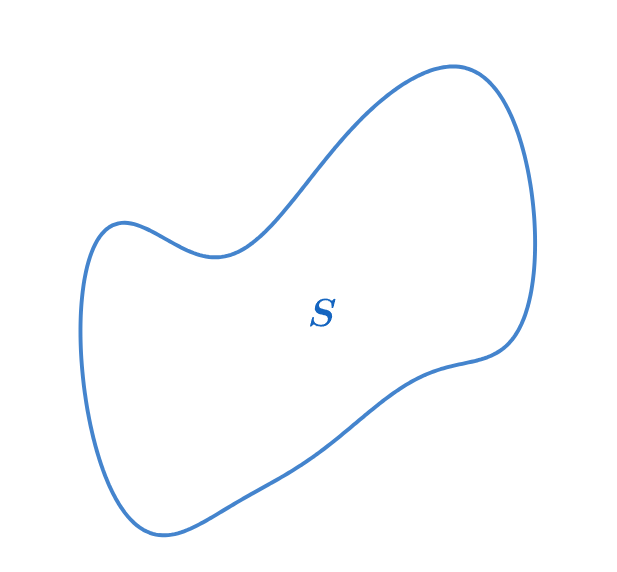
\includegraphics[height=7cm]{calculus/images/calculus_2024_02_07_0}
    \end{center}

    Надо найти ее площадь S

    Произведем ее дробление на маленькие элементарные фигуры, площадь которых мы можем посчитать:

    \begin{center}
        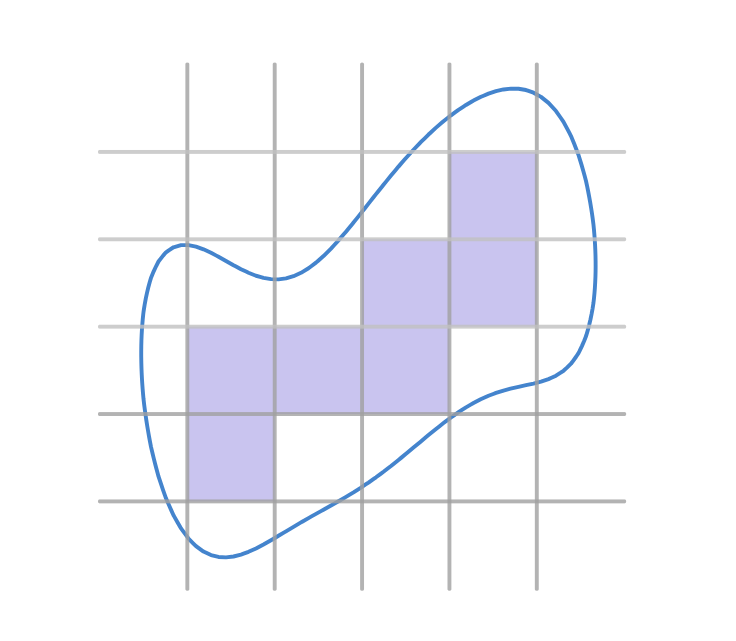
\includegraphics[height=7cm]{calculus/images/calculus_2024_02_07_1}
    \end{center}

    Уменьшаем дробление, чтобы свести погрешность к 0 (погрешность между истинной площадью и суммарной площадью прямоугольников)

    Сведем задачу к простейшей в ДПСК:

    \vspace{10mm}


    \begin{multicols}{2}
        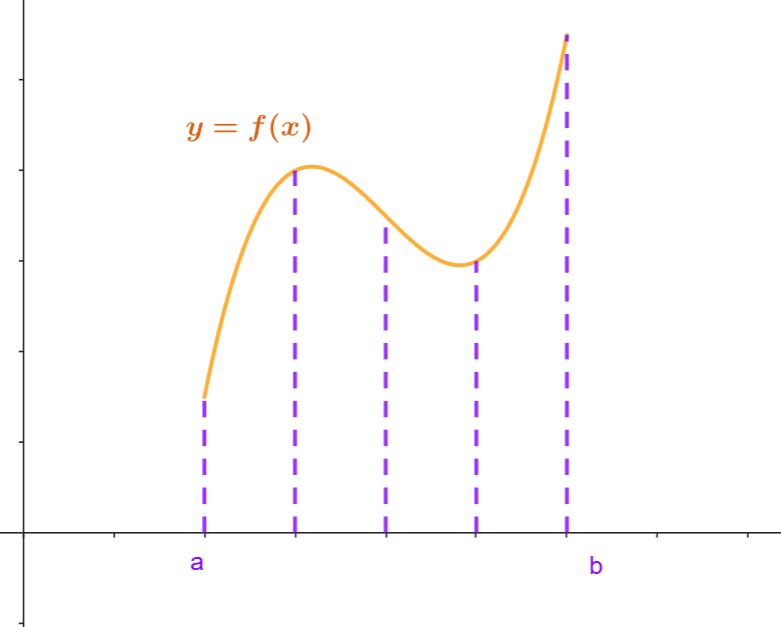
\includegraphics[height=6cm]{calculus/images/calculus_2024_02_07_2}

        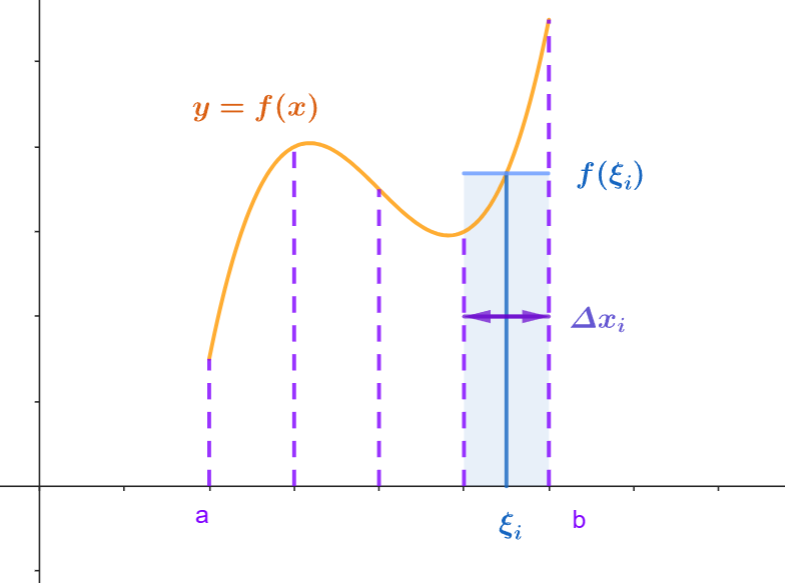
\includegraphics[height=6cm]{calculus/images/calculus_2024_02_07_3}
    \end{multicols}

    \begin{enumerate}
        \item Вводим разбиение отрезка $[a; b]\ (a < b)$ точками $a < x_0 < \dots < x_n < b$

        $T = \Set{x_i}^n_{i=0}$

        \item Выбираем средние точки на частичных отрезках $[x_{i-1}, x_i]^n_{i=1}$

        $\Set{\xi_i}_{i=1}^n$ - набор средних точек

        $\Delta x_i \stackrel{\text{обозн.}}{=} x_i - x_{i-1}$ - длина отрезка

        \item Строим элементарные прямоугольники
        \item Составляем сумму площадей всех таких прямоугольников:

        \[\sigma_n = \sum^n_{i=1} \Delta x_i f(\xi_i)\]

        - интегральная сумма Римана

        \item Заменяя разбиение, выбор $\xi_i$ при каждом $n$, получаем последовательность $\Set{\sigma_n}$

        При этом следим, чтобы ранг разбиения $\tau = \max\limits_{1 \leq i \leq n} \Delta x_i \rightarrow 0$ при $n \to \infty$

        Иначе получим неуничтожаемую погрешность

        \item \Def Если существует конечный предел интегральной суммы и он не зависит от типа,
        ранга дробления и выбора средних точек, то он называется определенным интегралом

        \[\lim_{n\to\infty,\ \tau\to0} \sigma_n = \lim_{n\to\infty,\ \tau\to0} \sum^n_{i=1} \Delta x_i f(\xi_i) \stackrel{\text{def}}{=} \int_a^b f(x)dx\]

    \end{enumerate}

    \Nota Независимость от дробления и выбора средних точек существенна

    \Ex $\mathcal{D} = \begin{cases}
                           1,\ x \in [0, 1], x \not\in \mathbb{Q} \\ 0,\ x \in [0, 1], x \in \mathbb{Q}
    \end{cases}$

    Сумма Римана для этой функции неопределенна, так как все зависит от выбора средних точек:
    \begin{itemize}
        \item если средние точки иррациональные, то сумма равна единице
        \item иначе сумма равна нулю
    \end{itemize}

    В обозначении определенного интеграла $a$ и $b$ называют нижним и верхним пределами интегрирования соответственно

    Дифференциал $dx$ имеет смысл $\Delta x$, понимается как б. м., то есть:

    $f(x) dx$ - площадь элементарных прямоугольников, тогда

    $\int^b_a f(x) dx$ - сумма этих прямоугольников

    \vspace{5mm}

    \begin{enumerate}
        \item $\int_a^a f(x)dx \stackrel{\text{def}}{=} 0$
        \item $\int_a^b f(x)dx = -\int_b^a f(x)dx$
    \end{enumerate}

    Можно доказать, что определенный интеграл существует для всякой непрерывной на отрезке функции

    \underline{Геом. смысл}. Заметим в определении площадь подграфика функции $(f(x) \geq 0)$

    Заметим, что для $f(x) \leq 0 \quad \int_a^b f(x)dx = -S$


    \section{1.2. Свойства}

    \begin{enumerate}
        \item Линейность пределов $\Longrightarrow$ линейность пределов

        $\lambda \int^b_a f(x)dx + \mu \int^b_a g(x)dx = \int^b_a (\lambda f(x) + \mu g(x)) dx \quad (\lambda, \mu \in \Real)$

        \item Аддитивность (часто для кусочно-непрерывных функций с конечным числом точек разбивается на участки непрерывности)

        $\int^b_a f(x)dx + \int^c_b f(x)dx = \int^c_a f(x)dx$

        Доказательства строятся на свойствах конечных сумм и пределов

        \item Оценка определенного интеграла

        $f(x)$ непрерывна на $[a; b]$ (имеет наимен. ($m$) и наибол. ($M$) значения). Тогда:

        $m (b-a) \leq \int^b_a f(x)dx \leq M(b - a)$

        $\Box$ Док-во:

        По теореме Вейерштрасса 2 $f(x)$ принимает наименьшее и наибольшее значения и для всякого $x$ из $[a; b]$:  $m <= f(x) <= M$

        Так как все средние точки принадлежат $[a; b]$, то

        $m \leq f(\xi_i) \leq M \quad \forall \xi_i$

        $m \Delta_i \leq f(\xi_i) \Delta_i \leq M \Delta_i$

        $m \sum_{i=1}^n \Delta x_i \leq f(\xi_i) \sum_{i=1}^n \Delta x_i \leq M \sum_{i=1}^n \Delta x_i$

        Предельный переход:

        $\lim_{n\to\infty,\ \tau\to0} m \sum_{i=1}^n \Delta x_i \leq \int^b_a f(x) dx \leq \lim_{n\to\infty,\ \tau\to0} M \sum_{i=1}^n \Delta x_i$

        $m \lim_{n\to\infty,\ \tau\to0} \sum_{i=1}^n \Delta x_i \leq \int^b_a f(x) dx \leq M \lim_{n\to\infty,\ \tau\to0} \sum_{i=1}^n \Delta x_i$

        $m (b - a) \leq \int^b_a f(x) dx \leq M (b - a)$

        $\Box$


        \item \Th Лагранжа о среднем (в интегральной форме)

        $f(x) \in C^\prime_{[a,b]} \Longrightarrow \exists \xi \in (a, b) \ f^\prime(\xi) = \frac{f(b) - f(a)}{b - a}$

        Тогда найдется такая средняя точка, что

        $f(x) \in C_{[a,b]} \Longrightarrow \exists \xi \in (a, b) \ f(\xi)(b - a) = \int^b_a f(x)dx$

        % help me

        $\Box$

        $m \leq \underset{\text{некоторое число}}{\undergroup{\frac{1}{b-a} \int_a^b f(x)dx}} \leq M$ по свойству выше

        По теореме Больцано-Коши $f(x)$ непрерывна, поэтому пробегает все значения от $m$ до $M$

        Значит найдется такая точка $\xi$, что $f(\xi) = \frac{1}{b-a} \int_a^b f(x)dx$

        $\Box$

        \item Сравнение интегралов

        $f(x), g(x) \in C_{[a, b]} \quad \forall x \in [a, b] \quad f(x) \geq g(x)$

        Тогда $\int_a^b f(x)dx \geq \int_a^b g(x)dx$

        $\Box$

        $\int_a^b f(x)dx - \int_a^b g(x)dx = \int_a^b (f(x) - g(x))dx =
        \lim_{n\to\infty,\ \tau\to0} \sum_{i=1}^n \underset{\geq 0}{\undergroup{(f(\xi_i) - g(\xi_i))}} \underset{\geq 0}{\undergroup{\Delta x_i}} \geq 0$

        $\Box$


        \item Интеграл и модуль

        $\left| \int^b_a f(x)dx \right| \leq \int^b_a |f(x)| dx$

        $\Box$

        $\int^b_a f(x)dx = \lim_{n\to\infty,\ \tau\to0} \sum_{i=1}^n f(\xi_i) \Delta x_i = \lim_{n\to\infty} \sigma_n$

        $\int^b_a |f(x)|dx = \lim_{n\to\infty,\ \tau\to0} \sum_{i=1}^n |f(\xi_i)| \Delta x_i$

        Докажем, что $\lim_{n\to\infty} |\sigma_n| = |\lim_{n\to\infty} \sigma_n|$

        Так как определен $\int^b_a f(x)dx = \lim_{n\to\infty} \sigma_n = S \in \Real$, то можно рассмотреть случаи

        $S > 0: \quad \exists n_0 \ \forall n > n_0 \ \sigma_n > 0$ (вблизи $S$)

        $\lim_{n\to\infty} |\sigma_n| = |\lim_{n\to\infty} \sigma_n|$

        $S > 0: \quad \exists n_0 \ \forall n > n_0 \ \sigma_n < 0$ (вблизи $S$)

        $\lim_{n\to\infty} |\sigma_n| = -\lim_{n\to\infty} \sigma_n = |\lim_{n\to\infty} \sigma_n|$

        $S = 0: \lim_{n\to\infty} |\sigma_n| = |\lim_{n\to\infty} \sigma_n| = 0$

        $\left| \int^b_a f(x)dx \left| = |\lim_{n\to\infty} \sigma_n| = \lim_{n\to\infty} |\sigma_n| =
        \lim_{n\to\infty,\ \tau\to0} \left|\sum_{i=1}^n f(\xi_i) \Delta x_i\right| \leq \lim_{n\to\infty,\ \tau\to0} \sum_{i=1}^n |f(\xi_i)| \Delta x_i$ (модуль суммы меньше или равен сумме модулей)

        $\Box$

    \end{enumerate}

    \Nota Интеграл и разрыв

    Изъятие из отрезка не более, чем счетного числа точек, не меняет значение интеграла, что позволяет считать интеграл на интервале

    \Nota Сходимость интеграла - в определении интеграла подчеркивается, что это число.
    Если предел интегральных сумм не существует или бесконечен, говорят, что интеграл расходится

    \Nota Вычисления

    Определение дает способ вычисления и его можно упростить:

    $\forall i\ \Delta x_i = \Delta x, \quad \xi_i = \begin{sqcases}
                                                         x_{i-1} \\ x_i
    \end{sqcases}$ - концы отрезка

    Так вычисляют \enquote{неберущиеся интегралы}

    Для функций, у которых первообразные выражаются в элементарных функциях используется не этот метод, а формула Ньютона-Лейбница


    \section{1.3. Вычисление определенного интеграла}


    \section{1.3.1. Интеграл с переменным верхним пределом}

    Дана $f(x): [a; +\infty), f(x) \in C_{[a; +\infty)}$

    $\forall x \in [a; +\infty)$ определен $\int^x_a f(x) dx$

    Таким образом определена функция $S(x) = \int_a^x f(x)dx$ - переменная площадь

    В общем случае обозначим $\Phi(x) = \int^x_a f(t) dt \quad t in [a, x]$

    Итак, различают три объекта:

    \begin{enumerate}
        \item Семейство функций: $\int f(x) dx = F(x) + C$
        \item Функция $\int^x_a f(t) dt = \Phi(x)$
        \item Число $\int^b_a f(x) dx = \lambda \in \Real$
    \end{enumerate}

    Выявим связь между ними.

    \Th Об интеграле с переменным верхним пределом (Барроу)

    $f(x) : [a;+\infty) \to \Real \quad f(x) \in C_{[a;+\infty+}$

    Тогда $\Phi(x) = \int^x_a f(t) dt$ - первообразная для $f(x)$ - $\Phi(x) = F(x)$

    $\Box$

    Докажем по определению

    $\Phi^\prime(x) = \lim_{\Delta x \to 0}\frac{\Delta \Phi}{\Delta x} = \lim_{\Delta x \to 0}\frac{\Phi(x + \Delta x) - \Phi(x)}{\Delta x} =
    \lim_{\Delta x \to 0}\frac{\int^{x + \Delta x}_a f(t)dt - \int^{x}_a f(t)dt}{\Delta x} =
    \lim_{\Delta x \to 0}\frac{\int^{x + \Delta x}_x f(t)dt}{\Delta x} = [\text{по \Ths Лагранжа } \exists \xi \in [x;x + \Delta x]] =
    \lim_{\Delta x \to 0} \frac{f(\xi)\Delta x}{\Delta x} = \lim_{\substack{\Delta x \to 0 \\ \xi \to x}} f(\xi) = f(x)$

    $\Box$

    \Th Основная теорема математического анализа (формула Ньютона-Лейбница, N-L)

    $f(x) \in C_{[a;b]}, F(x)$ - какая-либо первообразная $f(x)$

    \fbox{$\int^b_a f(x)dx = F(x) \Big|^b_a = F(b) - F(a)$}

    $\Box$

    Для $f(x)$ определена $\Phi(x) = \int_a^x f(t)dt = F(x) + C$

    Найдем значения $\Phi(a)$ и $\Phi(b)$

    $\Phi(a) = F(a) + C = \int^a_a f(t)dt = 0 \Longrightarrow F(a) + C = 0 \Longrightarrow F(a) = -C$

    $\Phi(b) = F(b) + C = F(b) - F(a) = \int^b_a f(t) dt$

    $\int^b_a f(x)dx = F(b) - F(a)$

    $\Box$


    \section{1.3.2. Методы интегрирования}

    1* Замена переменной в определенном интеграле

    \Th $f(x) \in C_{[a;b]} \quad x = \varphi(t) \in C^\prime_{[\alpha;\beta]}, \varphi(\alpha) = a, \varphi(\beta) = b$

    $\int^b_a f(x)dx = \int^\beta_\alpha f(\varphi(t)) \varphi^\prime(t) dt$

    $\Box$

    N-L: $\int^b_a f(x)dx = F(x) \Big|_a^b$

    Докажем, что $F(x) = F(\varphi(t))$ - первообразная для $f(\varphi(t))\varphi^\prime(t)$

    $\frac{dF(\varphi(t))}{dt} = F^\prime(\varphi(t)) \varphi^\prime(t)$

    $\frac{dF(\varphi(t))}{d\varphi(t)}\frac{d\varphi(t)}{dt} = \frac{dF(x)}{dx} \varphi^\prime(t) = f(x)\varphi^\prime(t)$

    $\Box$

    \Ex $\int_0^{\frac{1}{2}} \frac{dx}{\sqrt{1 - x^2}} = \begin{bmatrix}
                                                              x = \sin t \\ x \uparrow^\frac{1}{2}_0 \ t \uparrow_0^\frac{\pi}{6}
    \end{bmatrix} =
    \int_0^\frac{\pi}{6} \frac{dt}{\sqrt{1 - \sin^2 t}}\cos t =
    \int_0^\frac{\pi}{6} \frac{dt}{|\cos t|} \cos t = \int_0^\frac{\pi}{6} dt = t \Big|_0^\frac{\pi}{6} = \frac{\pi}{6}$

    2* По частям

    \Th $u, v \in C^\prime_{[a;b]} \quad uv \Big|_a^b = u(b)v(b) - u(a)v(a)$

    Тогда: $\int^b_a udv = uv \Big|_a^b - \int^b_a vdu$

    $\Box$

    $u(x)v(x)$ - первообразная для $u^\prime(x)v(x) + v^\prime(x)u(x)$

    Или $d(uv) = udv + vdu$

    По формуле N-L $\int_a^b (udv + vdu) = \int^b_a d(uv) = u(x)v(x) \Big|^b_a$

    $\int_a^b udv = uv \Big|^b_a - \int^b_a vdu$

    $\Box$

    \Ex $\int_1^e \ln x dx = x \ln x \Big|^e_1 - \int^e_1 xd\ln x = e \ln e - 1 \ln 1 -
    \int^e_1 dx = e - x \Big|_1^e = 1$

    \Nota Не всякий интеграл вида $\int^b_a f(x) dx $ является определенным

    \Ex $\int^e_0 \ln x dx = x \ln x \Big|_0^e - x \Big|_0^e = e \ln e - \underset{0 \cdot \infty}{\undergroup{0 \ln 0}} - e$ - несобственный интеграл



    \section{1.4. Приложения определенного интеграла}
    \hypertarget{integralapplications}{}

    \section{1.4.1. Площади}

    1* \Mem \hypertarget{integralareadpsk}{Значение интеграла} - площадь фигуры под графиком

    \begin{center}
        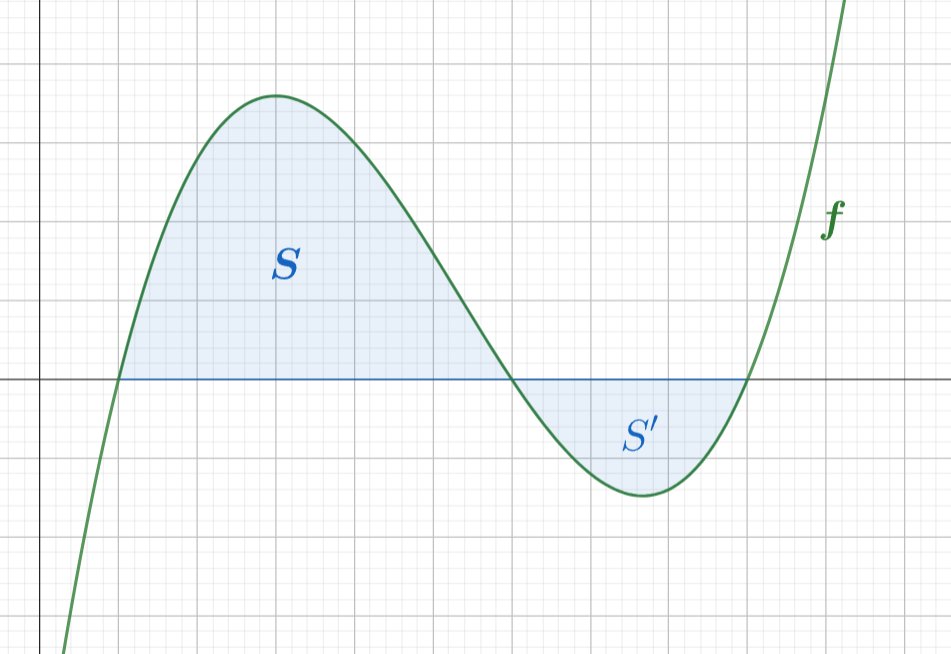
\includegraphics[height=6cm]{calculus/images/calculus_2024_02_14_1}
    \end{center}

    \underline{Геом. смысл}. $S = \int_a^b f(x) dx \quad\quad S^\prime = -\int_b^c f(x)dx$

    \mediumvspace

    2*

    \begin{center}
        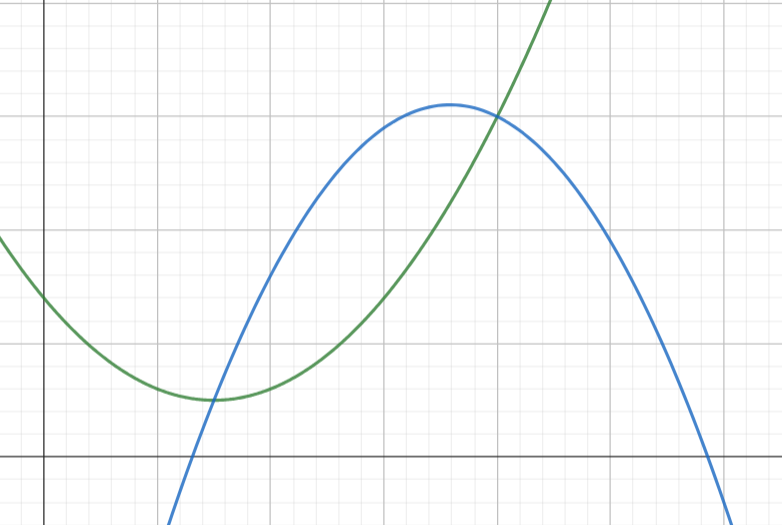
\includegraphics[height=6cm]{calculus/images/calculus_2024_02_14_3}
    \end{center}

    Площадь фигуры, окруженной графиками функций $S = \int_a^b |f(x) - g(x)| dx$, $a, b$ - абсциссы точек пересечения

    \Nota Симметрия

    Если $f(x)$ - четная функция, то $\int_{-a}^a f(x) dx = 2 \int_0^a f(x)dx$

    Если $f(x)$ - нечетная функция, то $\int_{-a}^a f(x) dx = 0$

    \section{1.4.2. Площадь в ПСК}

    \hypertarget{integralareapsk}{В ДПСК мы производили дробление фигуры на элементарные прямоугольники.} Сделаем подобное в ПСК для $\rho(\varphi)$:

    1) Дробление $[\alpha;\beta]$ на угловые сектора $[\varphi_{i - 1};\varphi_i]$

    $\Delta \varphi_i$ - угол сектора

    2) Выбор средней точки $\psi_i \in [\varphi_{i - 1};\varphi_i]$, площадь сектора $S_i = \frac{1}{2} \Delta \varphi_i \rho^2(\psi_i)$

    3) Интегральная сумма $\sigma_n = \frac{1}{2} \sum_{i=1}^n \rho^2 (\varphi_i) \Delta \varphi_i$

    4) Предел $\lim_{n \to \infty} \frac{1}{2} \sum_{i=1}^n \rho^2 (\varphi_i) \Delta \varphi_i = \frac{1}{2} \int_\alpha^\beta \rho^2(\varphi) d\varphi$

    \Ex Кардиоида:

    $\rho = 1 + \cos\varphi$

    $S = \frac{1}{2}\int^{\pi}_{-\pi} \rho^2 (\varphi) \Delta \varphi = \int_0^\pi \rho^2 (\varphi) \Delta \varphi =
    \int_0^\pi (1 + \cos\varphi)^2 \Delta \varphi = \int_0^\pi (1 + 2\cos\varphi + \cos^2\varphi) \Delta \varphi =
    \varphi \Big|_0^\pi + \int_0^\pi \frac{1 + \cos2\varphi}{2} \Delta \varphi = \pi + \frac{1}{2}\pi = \frac{3}{2}\pi$

    \Nota Если фигура задана параметрическими уравнениями:

    $\begin{cases}x = x(t) \\ y = y(t)\end{cases} \quad \alpha \leq t \leq \beta$

    То площадь будет равна $S = \int_a^b y(x)dx = \int^\beta_\alpha y(t)x^\prime(t)dt$

    \section{1.4.3. Длина кривой дуги}

    \hypertarget{lengthofarc}{Пусть дуга $AB$ задана уравнением $y = f(x) \quad x \in [a;b]$}

    \begin{enumerate}
        \item Производим дробление дуги на элементарные дуги точками $A = M_0 < M_1 < \dots < B = M_n$

        Здесь порядок $M_i$ таков, что их абсциссы $a = x_0 < x_1 < \dots < x_n = b \quad \Delta x_i > 0$

        \item Стягиваем сумму элементарными хордами. Сумма длин этих хорд при уменьшении их длин будет приближать длину этой дуги

        $\Delta s_i = \sqrt{\Delta y^2_i + \Delta x_i^2}$

        По \Ths Лагранжа существует такая точка $\xi_i \in [x_{i-1};x_i]$,
        что значение производной в этой точке равно наклону отрезка: $f^\prime(\xi_i) = \frac{f(x_i) - f(x_{i-1})}{x_i - x_{i-1}}$

        \item Интегральная сумма $\sigma_n = \sum_{i=1}^n \Delta s_i = \sum_{i=1}^n \sqrt{1 + (y^\prime(\xi_i))^2} \Delta x_i$

        \item Предельный переход $\lim_{\substack{n\to\infty \\ \tau \to 0}} \sigma_n = \int_a^b \sqrt{1 + (y^\prime(x))^2} dx = l_\text{дуги}$
    \end{enumerate}

    \Nota Очевидно потребовалась гладкость дуги, то есть спрямляемость. Только при этом условии $\Delta l_i \approx \Delta s_i$, и работает \Ths Лагранжа

    Параметрическое задание:

    $\begin{cases}x = \varphi(t) \\ y = \psi(t)\end{cases} \quad t \in [\alpha;\beta]$

    $\Delta s_i = \sqrt{(\Delta x_i)^2 + (\Delta y_i)^2} = \sqrt{(\varphi^\prime(\theta_i) \Delta t)^2 + (\psi^\prime(\theta_i) \Delta t)^2} =
    |\Delta t|\sqrt{(\varphi^\prime(\theta_i))^2 + (\psi^\prime(\theta_i))^2}$

    $l = \int^\beta_\alpha \sqrt{(\varphi^\prime(t))^2 + (\psi^\prime(t))^2} |dt|$

    \Ex Длина эллипса

    $L = 4l = 4 \int^\frac{\pi}{2}_0 \sqrt{a^2 \sin^2 t + b^2 \cos^2 t} dt =
    4 \int^\frac{\pi}{2}_0 \sqrt{(a^2 - b^2) \sin^2 t + b^2} dt =
    4 \int^\frac{\pi}{2}_0 \sqrt{c^2 \sin^2 t + b^2} dt = 4 \frac{b}{c} \int^\frac{\pi}{2}_0 \sqrt{1 + k^2 \sin^2 t} dt$ - эллиптический интеграл

    \section{1.4.4. Объемы тел}

    1* \hypertarget{volumeofbodieswithknownarea}{Объемы тел с известными площадями сечений}

    Для тела известна площадь сечения перпендикулярной $Ox$ плоскости $S(x)$

    Аналогично обычному дроблению $\lim_{\substack{n \to \infty \\ \tau \to 0}} \nu_n = \int^b_a S(x)dx = V_\text{тела}$

    \Ex Тело отсечено от I октанта плоскостью $\frac{x}{a} + \frac{y}{a} + \frac{z}{a} = 1$

    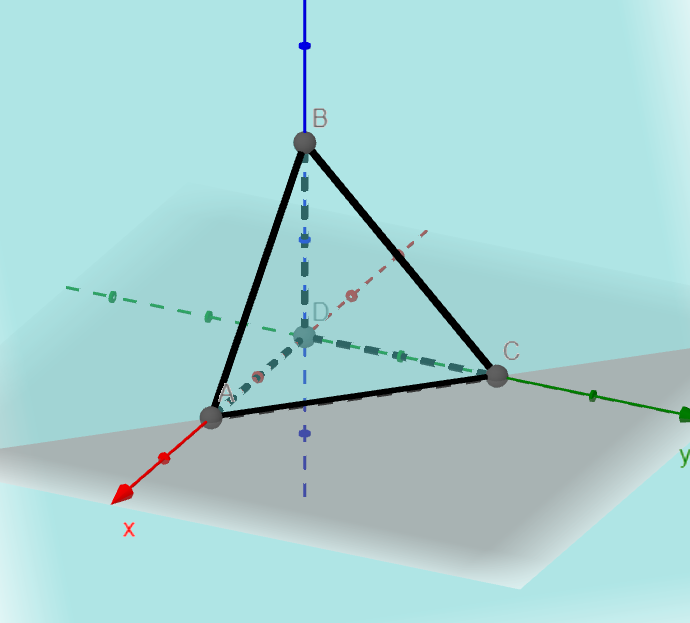
\includegraphics[height=7cm]{calculus/images/calculus_2024_02_14_2}

    $S(x) = S_{DBC} = \frac{(a - x)^2}{2}$

    Тогда $V = \int_0^a \frac{1}{2} (a - x)^2 dx = \frac{1}{2} \int_0^a (x - a)^2 dx =
    \frac{1}{2} \int^a_0 (x - a)^2 d(x - a) = \frac{1}{6} (x - a)^3 \Big|^a_0 = \frac{a^3}{6}$

    \Nota \hypertarget{volumeofbodyofrevolution}{Объем тела вращения}

    Пусть дана функция $r(x)$, задающая радиус тела вращения на уровне $x$,
    тогда объем тела вращения будет равен $\int_a^b \pi r^2(x) dx$

    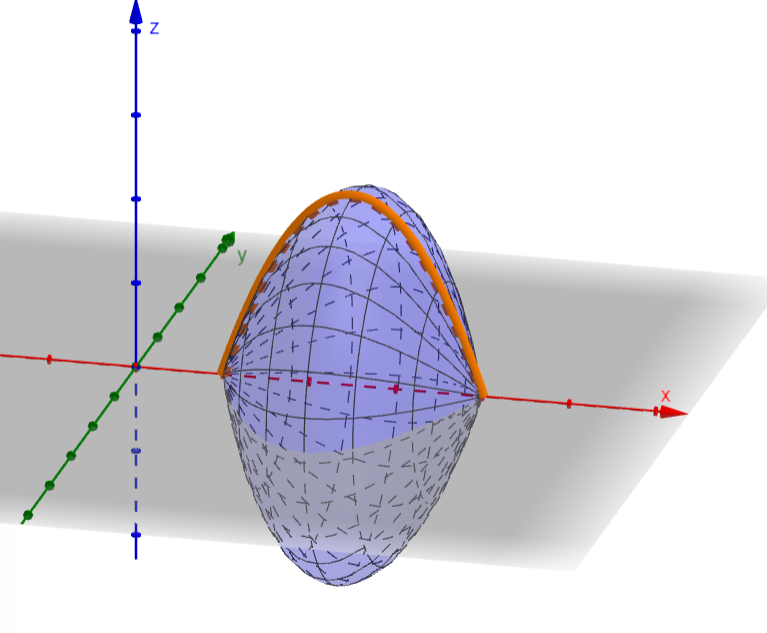
\includegraphics[height=7cm]{calculus/images/calculus_2024_02_14_4}



    \clearpage

    \section{2. Несобственные интегралы}

    \section{2.1 Определения}

    \textbf{1* Интегралы на неограниченном промежутке}

    Геометрический смысл: пусть $f(x) : [a; +\infty] \to \Real$, $f(x) \in C_{[a; +\infty]}$

    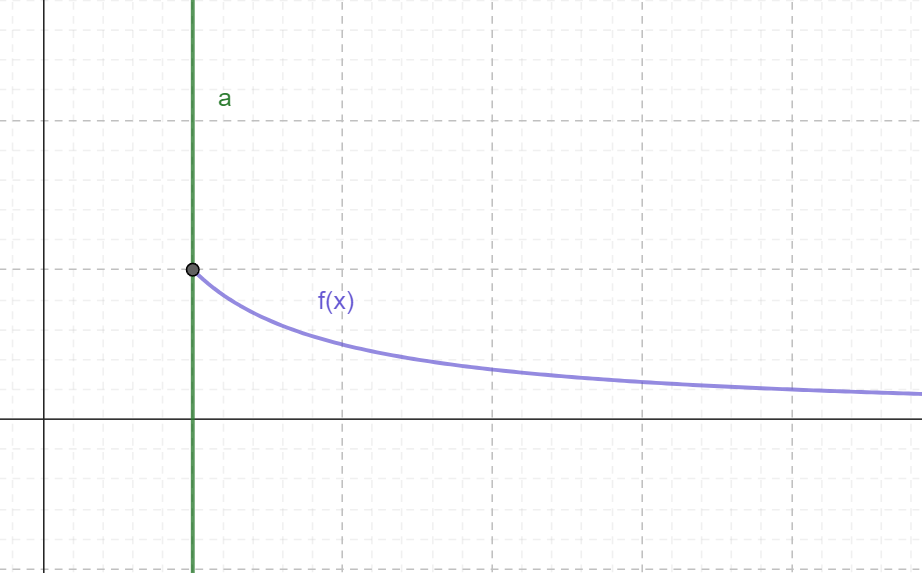
\includegraphics[height=90mm]{calculus/images/calculus_2024_02_21_1}

    Тогда определенный интеграл имеет смысл - это площадь под графиком функции:

    \[\int^{b}_{a} f(x) dx = S\]

    Имеет ли смысл площадь неограниченной фигуры под графиком функции?

    Предел функции $\Phi (b) = \int^{b}_{a} f(x) dx$ при $b \to +\infty$ может быть конечным или бесконечным

    \DefN{1} Определим несобственный интеграл первого рода (на неограниченном промежутке) ($f(x)$ любого знака):

    \[\int^{+\infty}_{a} f(x) dx = \lim_{b \to +\infty} \int^{b}_{a} f(x) dx\]

    \Nota Если этот предел существует и конечен, то говорят, что интеграл сходится. В противном случае расходится

    \DefN{2} Функция определена на полуинтервале $[-\infty; b]$ и непрерывна. Тогда определен:

    \[\int^{b}_{-\infty} f(x) dx = \lim_{a \to -\infty} \int^{b}_{a} f(x) dx\]

    \DefN{3} $\displaystyle \int^{+\infty}_{-\infty} f(x) dx = \int^{c}_{-\infty} f(x) dx + \int^{+\infty}_{c} f(x) dx$

    \Nota Этот интеграл сходится, если сходятся оба интеграла справа, и расходится, если расходится хотя бы один из них
    (в том числе если возникает неопределенность $\infty - \infty$)

    \Ex $f(x) = \frac{1}{x}$

    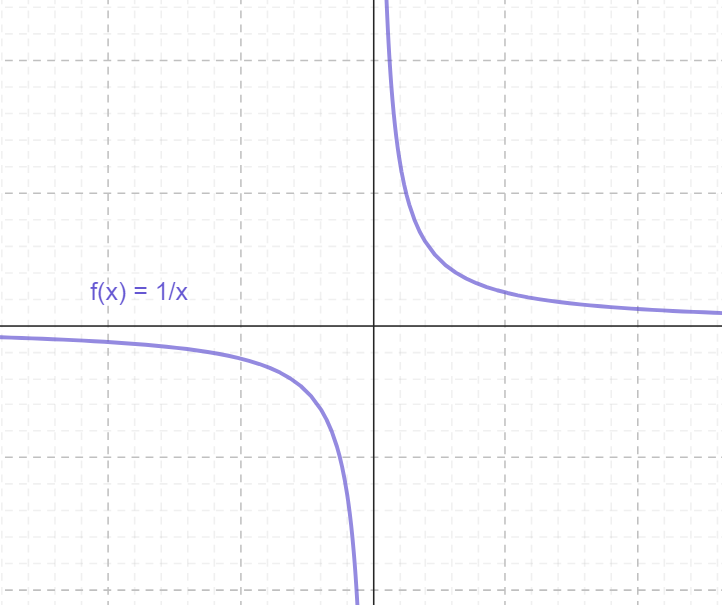
\includegraphics[height=90mm]{calculus/images/calculus_2024_02_21_2}

    Сделаем ее непрерывной

    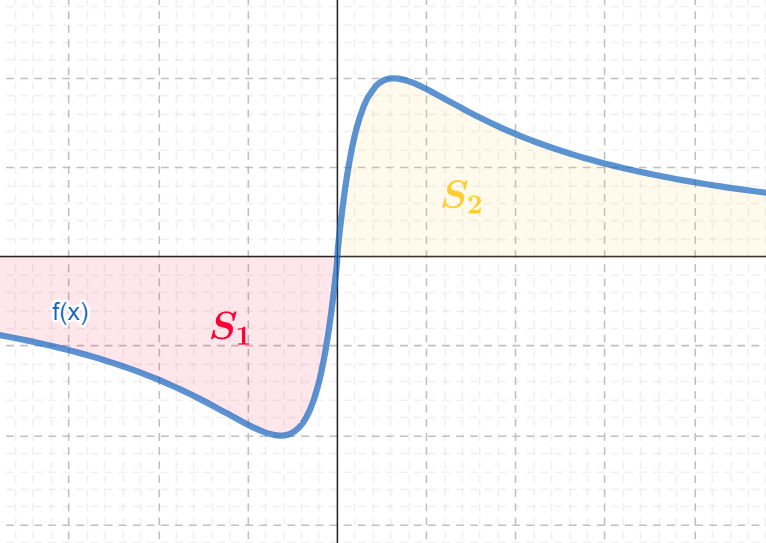
\includegraphics[height=90mm]{calculus/images/calculus_2024_02_21_3}

    $S_1 = S_2$, но $I_1 = -I_2$. Суммарный интеграл $\displaystyle \int^{+\infty}_{-\infty} f(x) dx$ должен быть равен нулю.

    Но по определению $\displaystyle \int^{+\infty}_{-\infty} f(x) dx$ расходится

    Чтобы учесть обнуление интеграла в ситуации взаимного погашения площадей $S_1$ и $S_2$
    (а это происходит тогда, когда левый и правый концы промежутка синхронно стремятся к $+\infty$)
    используют понятие интеграла в смысле главного значения ($v.p.$ - от французского \textit{valeur principale}):

    $\displaystyle v.p. \int^{+\infty}_{-\infty} f(x) dx = \lim_{\delta \to -\infty} \int^{\delta}_{-\delta} f(x) dx$

    Разложение по формуле Ньютона-Лейбница

    \ExN{1} \[\int^{+\infty}_{-\infty} \frac{dx}{1 + x^2} = arctg x \Big|^{+\infty}_{-\infty} = arctg x \Big|^{c = 0}_{-\infty} + arctg x \Big|^{+\infty}_{c = 0} =
    \lim_{x \to +\infty} arctgx - arctg(0) + arctg(0) - \lim_{x \to -\infty} arctgx = \frac{\pi}{2} + \frac{\pi}{2} = \pi\]

    \ExN{2} \[\int^{+\infty}_{1} \frac{dx}{xlnx} = \int^{+\infty}_{1} \frac{dlnx}{lnx} = \int^{+\infty}_{0} \frac{dt}{t}
     = lnt \Big|^{+\infty}_{0} = ln ln x \Big|^{+\infty}_{1} = \lim_{x \to +\infty} ln ln x - \lim_{x \to 1} ln ln x = \infty - \infty\] - расходится

    Заметим нарушение непрерывности функции $\frac{1}{xlnx}$ в $x = 1$, что привело к $ln lnx \to -\infty$ при $x \to 1$

    Это не интеграл первого рода, а комбинация интегралов первого и второго рода

    \textbf{2* Интеграл от неограниченной на отрезке функции}

    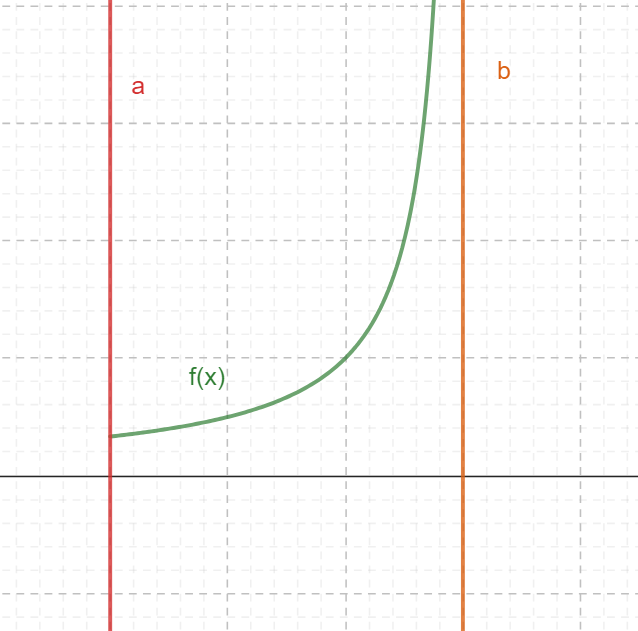
\includegraphics[height=90mm]{calculus/images/calculus_2024_02_21_4}

    $f(x) : [a; b) \to \Real$, где $b$ - точка разрыва второго рода, а именно бесконечного

    \DefN{1} Интеграл второго рода (несобственный)

    \[\int^{b}_{a} f(x) dx = \lim_{\beta \to b} \int^{\beta}_{a} f(x) dx\]

    Этот интеграл сходится, если предел существует и конечен

    \DefN{2} Аналогично ($a$ - точка бесконечного разрыва):

    \[\int^{b}_{a} f(x) dx = \lim_{\alpha \to a} \int^{b}_{\alpha} f(x) dx\]

    \DefN{3} $c \in [a;b]$ - точка бесконечного разрыва:

    \[\int^{b}_{a} f(x) dx = \int^{c}_{a} f(x) dx + \int^{b}_{c} f(x) dx\]

    Сходится, если оба интеграла сходятся

    \ExN{1}

    \[\int^{1}_{-1} \frac{dx}{x} = \int^{0}_{-1} \frac{dx}{x} + \int^{1}_{0} \frac{dx}{x} =
    ln |x| \Big|^{0}_{-1} + ln |x| \Big|^{1}_{0}\] - интеграл расходится

    Не заметили $\displaystyle \int^{1}_{-1} \frac{dx}{x} = ln |x| \Big|^{1}_{-1} = 0$ ???

    \ExN{2}

    \[\int^{1}_{-1} \frac{dx}{x^2} = -\frac{dx}{x} \Big|^{1}_{-1} = -2\] - неверно

    \[\int^{1}_{-1} \frac{dx}{x^2} = \int^{0}_{-1} \frac{dx}{x^2} + \int^{1}_{0} \frac{dx}{x^2} =
    -\frac{dx}{x} \Big|^{0}_{-1} + -\frac{dx}{x} \Big|^{1}_{0}\] - расходится

    \Nota Если нет разбиения $[a; b]$ по аддитивности, то неопределенности раскрываются

    \Ex $\int^{2}_{1} \frac{dx}{x^2 - 1} = \frac{1}{2} \int^{2}_{1} (\frac{1}{x - 1} - \frac{1}{x + 1})dx =
    \frac{1}{2} (ln|x - 1| - ln|x + 1|) \Big|^{2}_{1} = \\
    = \frac{1}{2} (ln|1 - 1| - ln|x + 1|) \Big|^{2}_{1} = \infty \text{,  т. к. разбивается отрезок}\\
    = \frac{1}{2} (ln|\frac{x - 1}{x + 1}) \Big|^{2}_{1} = \frac{1}{2} (ln\frac{1}{3} - ln(0)) = \infty \text{  - теперь точно } \infty
    $

    \section{2.2 Свойства}

    1) Линейность: $\displaystyle \int^{+\infty}_{a} (\lambda f(x) + \mu g(x)) dx = \lambda \int^{+\infty}_{a} f(x) dx + \mu \int^{+\infty}_{a} g(x) dx$
    - если интегралы сходятся (иначе исследуем по определению через предел)

    2) Аддитивность: $\displaystyle I = \int^{+\infty}_{a} f(x) dx = \int^{c}_{a} f(x) dx + \int^{+\infty}_{c} f(x) dx$
    - отсечение любого конечного интеграла $\int^{c}_{a} f(x) dx$ не влияет на сходимость

    3) Знаки интегралов:

    $\displaystyle \int^{+\infty}_{a} f(x) dx \geq \int^{+\infty}_{a} g(x) dx $ при $f(x) \leq g(x)$ и интегралы сходятся

    В частности $\displaystyle \int^{+\infty}_{a} f(x) dx \geq 0$ при $f(x) \leq 0$ на $[a; +\infty]$

    \Nota Исследование интегралов двух функций используется для определения их сходимости


    \section{2.3 Сходимость несобственных интегралов}

    Задача: Часто нужно исследовать интеграл на сходимость без или до его вычисления (обычно приближенного для неберущихся интегралов)

    Требуются признаки сходимости интегралов, часто использующие сравнение с эталонными интегралами (вычисляемые по формуле Ньютона-Лейбница)

    \textbf{2* Признак сравнения в неравенствах} (далее только для интегралов $\displaystyle \int^{+\infty}_{a} f(x) dx$, для остальных аналогично)

    $f(x), g(x) : [a;+\infty) \to \Real^+$, непрерывны на $[a;+\infty)$ и $\forall x \in [a;+\infty) f(x) \leq g(x)$


    Тогда, если $\displaystyle \int^{+\infty}_{a} g(x) dx = I \in \Real$, то $\displaystyle J = \int^{+\infty}_{a} f(x) dx$ сходится,
    причем $\displaystyle0 \leq \int^{+\infty}_{a} f(x) dx \leq \int^{+\infty}_{a} g(x) dx$

    Прежде чем использовать свойство ОИ и предельный переход в неравенства,
    нужно доказать, что интеграл $\displaystyle J = \lim_{b \to +\infty} \int^{b}_{a} f(x) dx$ сходится

    Т. к. $f(x) \geq 0$, то $\displaystyle \int^{b}_{a}f(x)dx$ при $b \to \infty$ монотонно возрастающая функция

    При этом:

    \[0 \leq \int^{b}_{a}f(x)dx \leq \int^{b}_{a}g(x)dx \leq \lim_{b \to +\infty} \int^{b}_{a}g(x)dx = I \in \Real\]

    То $\displaystyle J(b) = \int^b_a f(x)dx$ ограничена и по признаку Вейерштрасса сходится

    Можно использовать предельный переход

    \[0 \leq \int^{b}_{a}f(x)dx \leq \int^{b}_{a}g(x)dx \quad \Big| \lim_{b \to +\infty}\]

    \[0 \leq J \leq I\]

    \Nota Можно аналогично сравнить функции отрицательного знака

    Если сходится $\displaystyle \int^{+\infty}_{a} g(x) dx$ при $g(x) \leq f(x) \leq 0$, то сходится $\displaystyle \int^{+\infty}_{a} f(x) dx$

    Интегралы от функций разных знаков этим методов не сравниваются

    $f(x) \leq g(x) \forall x \in [a;+\infty)$, но функции разных знаков, и нижняя площадь, т. е. $\displaystyle \int^{b}_{a} |f(x)| dx$, больше верхней

    \textbf{1* $f(x), g(x) \in C_{[a;+\infty)}$, $0 \leq f(x) \leq g(x) \forall x \in [a;+\infty)$}

    $\displaystyle J = \int^{+\infty}_{a} f(x) dx \text{  расходится. Тогда  } I = \int^{+\infty}_{a} g(x) dx \text{  расходится}$

    $\Box$ \Lab (от противного)

    \Nota Отметим, что если $f(x)$ не является убывающей к нулю, т. е. б. м. на $+\infty$, то $\displaystyle \int^{+\infty}_{a} f(x) dx$ разойдется

    Таким образом, если сравнить б. м. $\displaystyle \frac{f(x)}{g(x)}$, то можно исследовать их интегралы на сходимость

    \textbf{2* Предельный признак сравнения}

    $f(x), g(x) \in C_{[a;+\infty)}$, $f(x), g(x) > 0$

    $\displaystyle \exists \lim_{x\to+\infty} \frac{f(x)}{g(x)} = k \in \Real \Setminus \Set{0}$.
    Тогда $\displaystyle I = \int^{+\infty}_{a} g(x)dx$ и $\displaystyle J = \int^{+\infty}_{a} f(x)dx$ одновременно сходятся или расходятся

    $\displaystyle \Box \lim_{x\to+\infty} \frac{f(x)}{g(x)} = k \Longleftrightarrow \forall \varepsilon > 0 \exists \delta > 0 | \forall x > \delta |\frac{f(x)}{g(x)} - k| < \varepsilon $

    $\displaystyle -\varepsilon + k < \frac{f(x)}{g(x)} < \varepsilon + k \quad \Big| * g(x) > 0$

    $\displaystyle (k - \varepsilon)g(x) < f(x) < (\varepsilon + k)g(x)$

    Т. к. $k > 0$ ($\frac{f(x)}{g(x)} > 0$) и $\varepsilon$ - сколь угодно мало, то $k \pm \varepsilon$ - положительное и не близкое к нулю число

    ОИ: $\displaystyle \int^{b}_{a} (k - \varepsilon)g(x) dx < \int^{b}_{a} f(x) dx < \int^{b}_{a} (k + \varepsilon)g(x) dx$

    $\displaystyle \lim_{b \to +\infty}$: $\displaystyle (k - \varepsilon) \int^{+\infty}_{a} g(x) dx < \int^{+\infty}_{a} f(x) dx < (k + \varepsilon) \int^{+\infty}_{a} g(x) dx$

    Если $I = \infty$ (но $k - \varepsilon \neq 0$), то по первому признаку (линейность) $J$ расходится
    Если $I \in \Real$ ($k + \varepsilon \neq \infty$), то по первому признаку (линейность) $J$ сходится

    \textbf{3* Абсолютная сходимость}

    $\displaystyle \int^{+\infty}_{a} |f(x)| dx = I \in \Real \Longrightarrow \int^{+\infty}_{a} f(x) dx = J \in \Real$

    \Nota Обратное неверно

    $\Box$ ОИ и модуль:

    \[\int^{b}_{a} f(x) dx \leq |\int^{b}_{a} f(x) dx| \leq \int^{b}_{a} |f(x)| dx\]

    Очевидно, что $\displaystyle 0 \leq |\int^{b}_{a} f(x) dx| \leq \int^{b}_{a} |f(x)| dx \leq \lim_{b \to \infty} \int^{b}_{a} |f(x)| dx = I$

    \[-I \leq \int^{b}_{a} f(x) dx \leq I\]

    \[0 \leq \lim_{b \to \infty}|\int^{b}_{a} f(x) dx| = |\lim_{b \to \infty} \int^{b}_{a} f(x) dx| \leq \int^{b}_{a} |f(x)| dx = I\]

    \Nota Если $\displaystyle I = \int^{+\infty}_{a} f(x) dx$ сходится, но $\displaystyle |\int^{+\infty}_{a} f(x) dx|$ расходится, то $I$ называют условно сходящимся

    \Ex $\displaystyle I = \int^{+\infty}_{a} \frac{sinx}{8x^2 + 3} dx$

    $\displaystyle \int^{+\infty}_{a} |\frac{sinx}{8x^2 + 3}| dx = \int^{+\infty}_{a} \frac{|sinx|}{8x^2 + 3} dx \text{синус ограничен} \leq \int^{+\infty}_{a} \frac{dx}{8x^2 + 3} dx = \frac{1}{k} arctg\frac{x}{k} \Big|^{+\infty}_{1} \in \Real$

    В качестве эталонных интегралов удобно использовать:

    I рода: $\displaystyle \int^{+\infty}_{a} \frac{dx}{x^n}$

    II рода: $\displaystyle \int^{b}_{a} \frac{dx}{(b - x)^n}$

    \Lab Исследовать на сходимость в зависимости от $n \in \Integer (\Rational)$

    \clearpage

    \section{3. Интегралы зависящие от параметра}

    Задача. Ex ($\alpha \neq 0$). $\displaystyle \int^{1}_{0} cos\alpha x dx = \frac{1}{\alpha} \int^{1}_{0} cos\alpha x d\alpha x = \frac{1}{\alpha} sin \alpha x \Big|^{1}_{0} = \frac{sin\alpha}{\alpha} = \phi(\alpha)$

    $\displaystyle J(\alpha) = \int^b_a f(x, \alpha)dx$ - интеграл, зависящий от параметра

    $f(x, \alpha)$ непрерывна в $a \leq x \leq b$, $c \leq \alpha \leq d$ и существует непрерывная производная $f^\prime_\alpha$

    Тогда на $[c;d]$ определена $J^\prime_\alpha(\alpha) = \left(\int^b_a f(x, \alpha)dx\right)^\prime_\alpha = \int^b_a f^\prime_\alpha dx$

    Если последний интеграл берется лучше, чем исходный, то теорема полезна

    $\displaystyle \Box J^\prime_\alpha(\alpha) = \lim_{\Delta \alpha \to 0} \frac{J(\alpha + \Delta \alpha) - J(\alpha)}{\Delta \alpha} =
    \lim_{\Delta \alpha \to 0} \frac{1}{\Delta \alpha} (\int^b_a f(x, \alpha + \Delta \alpha)dx - \int^b_a f(x, \alpha)dx) =
    = \lim_{\Delta \alpha \to 0} \frac{1}{\Delta \alpha} (\int^b_a (f(x, \alpha + \Delta \alpha) - f(x, \alpha))dx)$

    По теореме Лагранжа о среднем $\exists \xi \in [\alpha; \alpha + \Delta \alpha]$

    $\displaystyle = \lim_{\Delta \alpha \to 0} \int^b_a f(x, \xi)dx$

    Т. к. $f^\prime_\alpha$ непрерывна, то $\displaystyle f^\prime_\alpha (x, \xi) = \lim_{\xi \to \alpha} f^\prime_\alpha (x, \xi) + \varepsilon = f^\prime_\alpha (x, \alpha) + \varepsilon$

    Таким образом $\displaystyle J^\prime_\alpha(\alpha) = \lim_{\Delta \alpha \to 0} \int^{b}_{a} f^\prime_{\alpha}(x, \alpha) dx + \lim_{\Delta \alpha \to 0} \int^{b}_{a} \varepsilon dx =
    \lim_{\Delta \alpha \to 0} \int^{b}_{a} f^\prime_{\alpha}(x, \xi) dx$



    Теорема: $\displaystyle J^\prime_\alpha = \left(\int^b_a f(x, \alpha)dx\right)^\prime_\alpha = \int^b_a f^\prime_\alpha(x, \alpha)dx)$

    \Ex

    $\displaystyle I(\alpha) = \int^{+\infty}_0 e^{-x} \frac{sin\alpha x}{x}dx$
    $\displaystyle I^\prime_\alpha(\alpha) = \int^{+\infty}_0 (e^{-x} \frac{sin\alpha x}{x})^\prime_\alpha dx = \int^{+\infty}_0 e^{-x} \frac{1}{x} x cos\alpha x dx =
    \int^{+\infty}_0 e^{-x} cos\alpha x dx = \frac{1}{a + \alpha^2}$

    Из этого следует, что $\displaystyle I(\alpha) = \int_{+\infty}_{0} \frac{1}{a + \alpha^2} dx = arctg(\alpha) + C$

    Так как $I(\alpha)$ - несобственный интеграл, это функция, а не семейство функций. Найдем $C$.

    $\displaystyle I(0) = \int^{+\infty}_0 e^{-x} \frac{sin 0 * x}{x}dx = 0 \Longrightarrow C = 0$
    Таким образом, $\displaystyle I(\alpha) = (\int^{+\infty}_0 e^{-x} \frac{sin\alpha x}{x} dx)^\prime_\alpha = arctg(\alpha)$

    \Ex Гамма-функция

    \[\Gamma(\alpha) = \int^{+\infty}_0 x^{\alpha - 1} e^{-x} dx \quad (\alpha > 0)\]

    Исследуем на сходимость:

    \[\Gamma(\alpha) = \int^{+\infty}_0 x^{\alpha - 1} e^{-x} dx = \int^{1}_0 x^{\alpha - 1} e^{-x} dx + \int^{+\infty}_1 x^{\alpha - 1} e^{-x}\]

    На отрезке $[0; 1]$ $e^(-x) \in [0;1]$.
    Тогда $\displaystyle 0 \leq \int^{1}_0 x^{\alpha - 1} e^{-x} dx \leq \int^{1}_0 x^{\alpha - 1} dx \Longrightarrow$ интеграл сходится

    Пусть $n > \alpha - 1, n \in \Natural$, тогда:

    $\displaystyle \int^{+\infty}_1 x^{\alpha - 1} e^{-x} dx \leq \int^{+\infty}_1 x^{n} e^{-x} dx$ - по частям, появятся $\dislpaystyle x^{k} e^{-x} \Big|^{+\infty}_1 \rightarrow 0$ и $\dislpaystyle \int^{+\infty}_1 e^{-x} dx$ сходится

    Найдем формулу для $\Gamma(\alpha)$:

    $\displaystyle \alpha \in \Natural \quad \Gamma(1) = \int^{+\infty}_0 e^{-x} dx = -e^{-x} \Big|^{+\infty}_{0} = 1$

    $\displaystyle \Gamma(\alpha) = \int^{+\infty}_0 x^{\alpha - 1} e^{-x} dx = -\int^{+\infty}_0 x^{\alpha - 1} de^{-x} = -x^{\alpha - 1}e^{-x} \Big|^{+\infty}_1 + \int^{+\infty}_0 x^{\alpha - 2} (\alpha - 1) e^{-x} dx = (\alpha - 1) \Gamma(\alpha - 1) = $
    $(\alpha - 1)! \Gamma(1) = (\alpha - 1)!$

    $\Gamma(n + 1) = n!$

    \Lab Посмотреть, как обобщается понятие факториала на вещественные числа:

    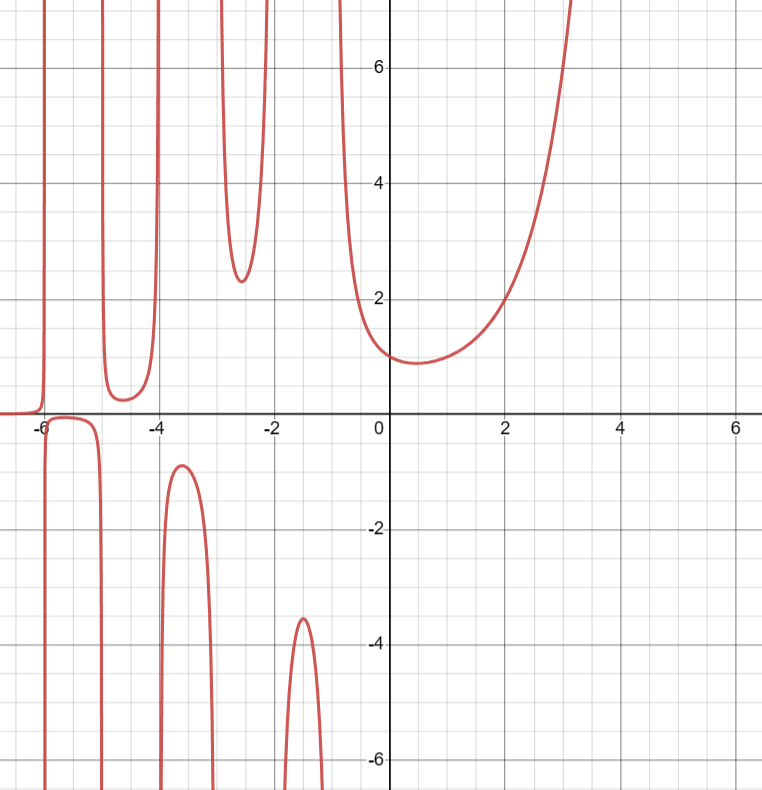
\includegraphics[height=70mm]{calculus/images/calculus_2024_02_28_1}

    \clearpage

    \section{4. Функция нескольких переменных (ФНП)}

    \section{4.1. Определение}

    \Nota Дадим определение ФНП

    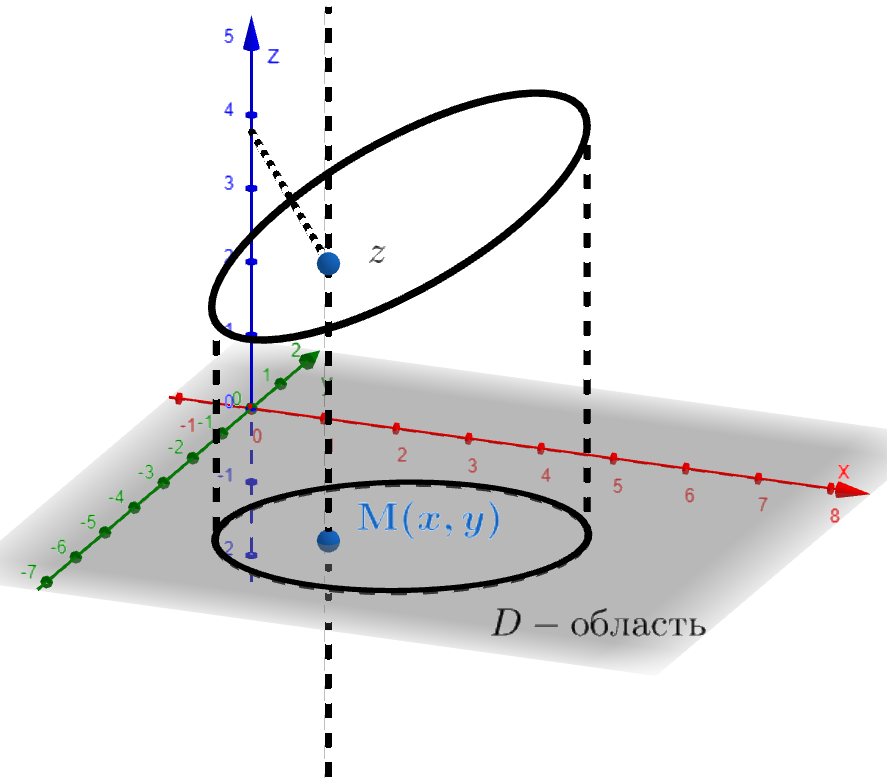
\includegraphics[height=90mm]{calculus/images/calculus_2024_02_28_2}

    $\forall M(x, y) \exists! z \in \Real : z = f(x, y) \Longleftrightarrow z = f(x, y)$ - функция двух переменных

    \Def Окрестность точки $M_0(x_0, y_0)$

    $U_\delta (M_0) = \Set{(x, y) \in Oxy : (x - x_0)^2 + (y - y_0)^2 < \delta^2, \delta > 0 \text{ - радиус}}$

    $\stackrel{o}{U}_\delta (M_0)$ - выколотая

    \Nota $\Delta x = x - x_0, \Delta y = y - y_0$, одновременное стремление $\Delta x, \Delta y \rightarrow 0$
    можно заменить $\Delta \pho = \sqrt{(x - x_0)^2 + (y - y_0)^2} \rightarrow 0$\\[1\baselineskip]


    \Def $\displaystyle \lim_{M \to M_0} z(x, y) = L \in \Real \Longleftrightarrow \forall \varepsilon > 0 \exists \delta > 0 (\delta = \delta(\varepsilon)) | \forall M \in \stackrel{o}{U}_\delta(M_0) \text{ } |z(x, y) - L| < \varepsilon$

    $M_0$ - точка сгущения и $x_0, y_0 \in \Real$ (здесь)

    \Nota На плоскости $Oxy$ возможно стремление $M \rightarrow M_0$ по разным путям $F(x, y) = 0$ (уравнение кривой)

    При этом значение предела вдоль разных путей могут отличаться (аналог односторонних пределов)

    Предел в определении - предел в общем смысле: его существование и значение не зависит от пути

    \Def $z = f(x, y)$ называется непрерывной в точке $M_(x_0, y_0)$, если $z = f(x_0, y_0) = \lim_{M \to M_0} z(x, y)$

    $z$ непрерывна на $D$, если $z$ непрерывна $\forall (x, y) \in D$

    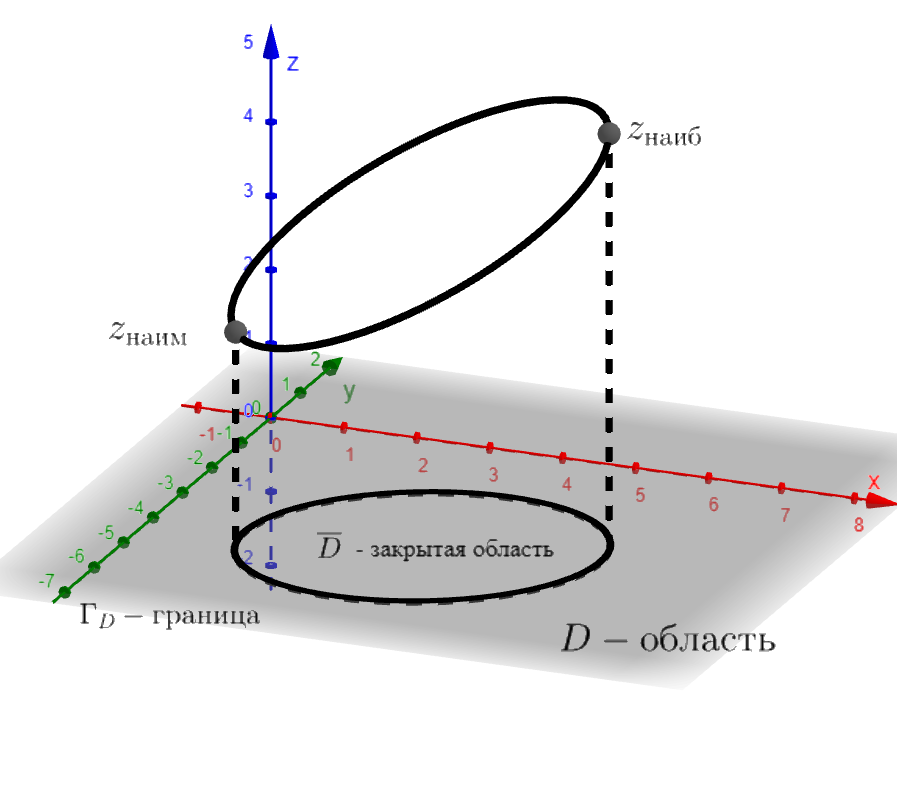
\includegraphics[height=90mm]{calculus/images/calculus_2024_02_28_3}

    \Nota Справедливы теоремы Вейерштрасса и Больцано-Коши для функции, непрерывной в заданной области

    $z = f(x, y)$ непрерывна на $\overline{D} = D \union \Gamma_D$, где $\overline{D}$ - закрытая область, $D$ - открытая область, $\Gamma_D$ - граница

    \ThN{W1} $z = f(x, y)$ ограничена на $\overline{D}$

    \ThN{W2} $\exists$ наибольшее и наименьшее $z \in \overline{D}$

    \ThN{B-C1} на границе $\Gamma_D$ $z$ принимает значения разных знаков $\Longrightarrow \exists M \in \overline{D} : z(M) = 0$

    \ThN{B-C1} $z(x, y)$ принимает все значения от $z_{\text{наим}}$ до $z_{\text{наиб}}$ \\[1\baselineskip]

    \section{4.2. Производные функции двух переменных}

    Путям $l_1, l_2$ соответствуют кривые $L_1, L_2$ на поверхности $z = f(x, y)$.

    Пользуясь геометрическим смыслом производной, заметим, что касательные к $L_1, L_2$ могут быть различными.


    Поэтому для определения производной выберем координатные направления $x = const$ и $y = const$

    $z = f(x = c, y)$

    $\displaystyle \frac{\partial z}{\partial y} \stackrel{def}{=} \lim_{\Delta y \to 0} \frac{\Delta_y z}{\Delta y}$,
    где $\Delta_y z = z(x, y + \Delta y) - z(x, y)$

    Определили частную производную $z$ по $y$

    \Lab Дать определение $\displaystyle \frac{\partial z}{\partial x}$

    \Nota $\Delta_y z = z(x, y + \Delta y) - z(x, y)$ и  $\Delta_y z$ называют частным приращением

    \Def Полное приращение $\Delta z \stackrel{def}{=} z(x + \Delta x, y + \Delta y) - z(x, y)$

    \Nota $\Delta z \neq \Delta_x z + \Delta_y z$ !!!

    Обозн.: $\displaystyle \frac{\partial z}{\partial x} = z^\prime_x = z_x$, $\displaystyle \frac{\partial z}{\partial y} = z^\prime_y = z_y$

    Как определить функцию, дифференцируемую в точке?

    По аналогии $\Delta z = A \Delta x + B \Delta y + \alpha \Delta x + \beta \Delta y$, где $A, B \in \Real$, $\alpha, \beta$ - б. м.



    Дифференциал

    \Th $\displaystyle z : D \rightarrow \Real, \ D \subset \Real^2, \ \exists$
    непрерывные $\displaystyle \frac{\partial z}{\partial x}$, $\displaystyle \frac{\partial z}{\partial y}$

    Тогда функция представима $\displaystyle \Delta z = A dx + B dy + \alpha \Delta x + \beta \Delta y$, где $\displaystyle A, B \in \Real, \ \alpha, \beta = $ б. м.

    $\displaystyle \Box \quad \Delta z = z (x + \Delta x, y + \Delta y) - z (x, y) = z(x + \Delta x, y + \Delta y) - z(x + \Delta x, y) +
    z(x + \Delta x, y) - z(x, y)$

    По теореме Лагранжа:

    $\displaystyle z(x + \Delta x, y + \Delta y) - z(x + \Delta x, y) = z^\prime_y(\eta) \Delta y$

    $\displaystyle z(x + \Delta x, y) - z(x, y) = z^\prime_x(\xi)\Delta x$

    По теореме о представлении функции ее пределом:

    $\displaystyle z^\prime_x(\xi) = \lim_{\xi \to x (\Delta x \to 0)} z^\prime_x(\xi) + \alpha$

    $\displaystyle z^\prime_y(\eta) = \lim_{\eta \to y} z^\prime_y(\eta) + \beta$

    Так как $\displaystyle z^\prime_x(\xi), z^\prime_y(\eta)$ непрерывны, то $\displaystyle \lim_{\xi \to x} z^\prime_x(\xi) = \frac{\partial z}{\partial x}, \lim_{\eta \to y} z^\prime_y(\eta) = \frac{\partial z}{\partial y}$

    Тогда $\displaystyle \Delta z = \left(\frac{\partial z}{\partial x} + \alpha\right) \Delta x + \left(\frac{\partial z}{\partial y} + \beta\right)\Delta y =
    \Delta z = \frac{\partial z}{\partial x}\Delta x + \frac{\partial z}{\partial y}\Delta y + \alpha \Delta x + \beta \Delta y$

    Заметим, что $\displaystyle \alpha \Delta x$ и $\displaystyle \beta \Delta y$ - б. м. порядка выше, чем $\displaystyle \Delta \rho = \sqrt{(\Delta x)^2 + (\Delta y)^2} \Longleftrightarrow$

    $\displaystyle 1 = \sqrt{\left(\frac{\Delta x}{\Delta \rho}\right)^2 + \left(\frac{\Delta y}{\Delta \rho}\right)^2} \quad |\frac{\Delta x}{\Delta \rho}| \leq 1, |\frac{\Delta y}{\Delta \rho}| \leq 1$

    Сравним $\displaystyle \frac{\alpha \Delta x}{\Delta \rho} =$ б. м. огр. $\displaystyle \stackrel{\Delta \rho \to 0}{\to} 0$, $\displaystyle \frac{\beta \Delta y}{\Delta \rho} \stackrel{\Delta \rho \to 0}{\to} 0$

    Функция, приращение которой представимо $\displaystyle \Delta z = \frac{\partial z}{\partial x}\Delta x + \frac{\partial z}{\partial y}\Delta y + o(\Delta \rho)$, называется дифференцируемой в точке $\displaystyle (x, y)$,
    линейная часть приращения называется полным дифференциалом

    Обозначение: $\displaystyle dz = \frac{\partial z}{\partial x} dx + \frac{\partial z}{\partial y} dy$

    \Ex $\displaystyle z = 3xy^2 + 4cosxy$

    $\displaystyle \frac{\partial z}{\partial x} \stackrel{y = const}{=} 3y^2 - 4sinxy \cdot y$

    $\displaystyle \frac{\partial z}{\partial y} \stackrel{x = const}{=} 6xy - 4sinxy \cdot x$

    $\displaystyle dz = (3y^2 - 4ysinxy)dx + (6xy - 4xsinxy)dy$
    
    \vspace{8mm}

    \section{4.3. Правила дифференцирования}

    \Nota При нахождении $\displaystyle \frac{\partial z}{\partial x_i}$ ($x_i$ - какая-либо переменная) дифференцирование проводится по правилам для функции одной переменной ($x_j \neq x_i$ считаются константами)

    Выпишем более сложные правила
    
    \vspace{3mm}

    \textbf{1* Сложная функция}

    \Mem $\displaystyle (f(g(x)))^\prime = f^\prime(g(x)) \cdot g^\prime(x)$

    \Def Сложная функция двух переменных: $\displaystyle z = z(u, v), u = u(x, y), v = v(x, y)$

    Формула: Найдем $\displaystyle frac{\partial z(u, v)}{\partial x}$ и $\displaystyle frac{\partial z(u, v)}{\partial y}$

    \Th $\displaystyle z = z(u, v), \ u(x, y), v(x, y)$ непрерывно дифференцируемы по $\displaystyle x, y$

    Тогда $\displaystyle \frac{\partial z}{\partial x} = \frac{\partial z}{\partial u} \cdot \frac{\partial u}{\partial x} + \frac{\partial z}{\partial v} \cdot \frac{\partial v}{\partial x}$
    $\displaystyle \frac{\partial z}{\partial y} = \frac{\partial z}{\partial u} \cdot \frac{\partial u}{\partial y} + \frac{\partial z}{\partial v} \cdot \frac{\partial v}{\partial y}$

    $\displaystyle \Box \quad z$ дифференцируема $\displaystyle \Longleftrightarrow \Delta z = \frac{\partial z}{\partial u} \Delta u + \frac{\partial z}{\partial v} \Delta v + \alpha \Delta u + \beta \Delta v$

    Зададим приращение $\displaystyle \Delta x$ (представление $\displaystyle \Delta z$ не должно измениться)

    $\displaystyle \Delta_x z = \frac{\partial z}{\partial u} \Delta_x u + \frac{\partial z}{\partial v} \Delta_x v + \alpha \Delta_x u + \beta \Delta_x + v \quad \Big| \cdot \Delta x$

    $\displaystyle \frac{\Delta_x z}{\Delta x} = \frac{\partial z}{\partial u} \frac{\Delta_x u}{\Delta x} + \frac{\partial z}{\partial v} \frac{\Delta_x v}{\Delta x} + \alpha \frac{\Delta_x u}{\Delta x} + \beta \frac{\Delta_x v}{\Delta x} \quad \Big| \cdot \Delta x$

    По теореме Лагранжа: $\displaystyle \frac{\partial u}{\partial x}(\xi) \stackrel{\Delta x \to 0}{\rightarrow} \frac{\partial u}{\partial x}$

    В пределе: $\displaystyle \frac{\partial z}{\partial x} = \frac{\partial z}{\partial u} \frac{\partial u}{\partial x} + \frac{\partial z}{\partial v} \frac{\partial v}{\partial x}$

    Аналогично для $\displaystyle \frac{\partial z}{\partial y}$

    \Nota Интересен случай $\displaystyle z = z(x, u, v)$, где $\displaystyle u = u(x), v = v(x)$

    Здесь $\displaystyle z$ является функцией одной переменной $\displaystyle x$

    Обобщая правило на случай трех переменных, можем записать формулу полной производной, которая имеет смысл

    $\displaystyle \frac{dz}{dx} = \frac{\partial z}{\partial x} \cdot \frac{\partial x}{\partial x} +
    \frac{\partial z}{\partial u} \cdot \frac{\partial u}{\partial x} +
    \frac{\partial z}{\partial v} \cdot \frac{\partial v}{\partial x} =
    \frac{\partial z}{\partial x} +
    \frac{\partial z}{\partial u} \cdot \frac{du}{dx} +
    \frac{\partial z}{\partial v} \cdot \frac{dv}{dx}
    $\displaystyle 

    \Ex Пусть $\displaystyle w = w(x, y, z)$ - функция координат $\displaystyle x = x(t), y = y(t), z = z(t)$ - функции времени

    $\displaystyle w$ явно не зависит от времени, тогда $\displaystyle \frac{dw}{dt} = w^\prime_x v_x + w^\prime_y v_y + w^\prime_z v_z$, где $\displaystyle v_x$ - проекция скорости

    Если $\displaystyle w = w(x, y, z, t)$, то $\displaystyle \frac{dw}{dt} = \frac{\partial w}{\partial t} w^\prime_x v_x + w^\prime_y v_y + w^\prime_z v_z$
    
    \vspace{3mm}
    
    \textbf{2* Неявная функция одной переменной}: пусть $\displaystyle F(x, y(x)) = 0$ - неявное задание $\displaystyle y = y(x)$

    Найдем $\displaystyle dF = \frac{\partial F}{\partial x} dx + \frac{\partial F}{\partial y} dy = 0$

    Отсюда $\displaystyle \frac{dy}{dx} = -\frac{\frac{\partial F}{\partial x}}{\frac{\partial F}{\partial y}}$
    
    \vspace{8mm}

    \section{4.4. Производная высших порядков}

    \Nota Пусть $\displaystyle z = z(x, y)$ дифференцируема и $\displaystyle \frac{\partial z}{\partial x}, \frac{\partial z}{\partial y}$ также дифференцируемы, при этом в общем случае
    $\displaystyle \frac{\partial z}{\partial x} = f(x, y), \frac{\partial z}{\partial y} = g(x, y)$

    Тогда определены вторые частные производные
    
    \vspace{3mm}

    \Def $\displaystyle \frac{\partial^2 z}{\partial x^2} \stackrel{def}{=} \frac{\partial}{\partial x} \frac{\partial z}{\partial x}$

    $\displaystyle \frac{\partial^2 z}{\partial y^2} = \frac{\partial}{\partial y} \frac{\partial z}{\partial y}$ - чистые производные


    $\displaystyle \frac{\partial^2 z}{\partial x \partial y} = \frac{\partial}{\partial y} \frac{\partial z}{\partial x}$

    $\displaystyle \frac{\partial^2 z}{\partial y \partial x} = \frac{\partial}{\partial x} \frac{\partial z}{\partial y}$ - смешанные производные

    \vspace{3mm}

    \Th $\displaystyle z = z(x, y)$, функции $\displaystyle z(x, y), z^\prime_x, z^\prime_y, z^{\prime\prime}_{xy}, z^{\prime\prime}_{yx}$ определены и непрерывны в $\displaystyle \stackrel{o}{U}(M(x, y))$

    Тогда $\displaystyle z^{\prime\prime}_{xy} = z^{\prime\prime}_{yx}$

    $\displaystyle \Box \quad$ Введем вспомогательную величину

    $\displaystyle \Phi = (z(x + \Delta x, y + \Delta y) - z(x + \Delta x, y)) - (z(x, y + \Delta y) - z(x, y))$

    Обозначим $\displaystyle \phi(x) = z(x, y + \Delta y) - z(x, y)$

    Тогда $\displaystyle \Phi = \phi(x + \Delta x) - \phi(x)$ - дифференцируема, непрерывна, как комбинация

    По теореме Лагранжа $\displaystyle \phi(x + \Delta x) - \phi(x) = \phi^\prime(\xi) \Delta x = (z^\prime_x(\xi, y + \Delta y) - z^\prime_x(\xi, y)) \Delta x$, где $\displaystyle \xi \in (x; x + \Delta x)$

    Здесь $\displaystyle z^\prime_x$ дифференцируема также на $\displaystyle [y, y + \Delta y]$


    Тогда по теореме Лагранжа $\displaystyle \exists \eta \in (y, y + \Delta y) \ | \ z^\prime_x(\xi, y + \Delta y) - z^\prime_x(\xi, y) = z^{\prime\prime}_{xy} (\xi, \eta) \Delta y$

    Таким образом $\displaystyle \Phi = z^{\prime\prime}_{xy} (\xi, \eta) \Delta x \Delta y$

    Перегруппируем $\displaystyle \Phi$, далее аналогично для $\displaystyle z^{\prime\prime}_{yx}$

    Тогда $\displaystyle z^{\prime\prime}_{xy} (\xi, \eta) \Delta x \Delta y = \Phi = z^{\prime\prime}_{yx} (\xi^\prime, \eta^\prime) \Delta x \Delta y$

    \vspace{8mm}

    \section{4.5. Дифференциалы}
    
    \MemN{1} Полный дифференциал (1-ого порядка) функции $\displaystyle z = z(x, y)$

    $\displaystyle dz = \frac{\partial z}{\partial x} dx + \frac{\partial z}{\partial y} dy$ - сумма частных дифференциалов

    \MemN{2} Инвариантность формы первого дифференциала функции одной переменной

    $\displaystyle dy(x) = y^\prime(x)dx \stackrel{x = \phi(t)}{=} y^\prime(t)dt$

    \vspace{3mm}
    
    \Th Инвариантность полного дифференциала первого порядка.

    $\displaystyle z = z(u, v), \quad u = u(x, y), \quad v = v(x, y)$ - дифференциалы

    Тогда $\displaystyle dz = \frac{\partial z}{\partial u}du + \frac{\partial z}{\partial v} dv = \frac{\partial z}{\partial x} dx + \frac{\partial z}{\partial y} dy$

    $\displaystyle \Box \quad dz = \frac{\partial z}{\partial u} \left(\frac{\partial u}{\partial x} dx + \frac{\partial u}{\partial y} dy\right) +
    \frac{\partial z}{\partial v} \left(\frac{\partial v}{\partial x} dx + \frac{\partial v}{\partial y} dy\right) =
    \left(\frac{\partial z}{\partial u} \frac{\partial u}{\partial x} + \frac{\partial z}{\partial v} \frac{\partial v}{\partial x}\right) dx +
    \left(\frac{\partial z}{\partial u} \frac{\partial u}{\partial y} + \frac{\partial z}{\partial v} \frac{\partial v}{\partial y}\right) dy =
    \frac{\partial z}{\partial x} dx + \frac{\partial z}{\partial y} dy$


    \Mem $\displaystyle d^2 y(x) \stackrel{def}{=} d(dy(x)) = y^{\prime\prime}(x) dx^2 \neq y^{\prime\prime}(t) dt^2$

    \vspace{3mm}
    
    \textit{Def}: $\displaystyle z = z(x, y)$ - дифференцируема и $\displaystyle dz = \frac{\partial z}{\partial x}dx + \frac{\partial z}{\partial y}dy$ - дифференцируемая функция

    Тогда второй полный дифференциал:

    $\displaystyle d^2 z \stackrel{def}{=} d(dz)$

    Формула: $\displaystyle d^2 z = d\left(\frac{\partial z}{\partial x}dx + \frac{\partial z}{\partial y}dy\right) = (z^\prime_x dx + z^\prime_y dy)^\prime_x dx + (z^\prime_x dx + z^\prime_y dy)^\prime_y dy =
    (z^\prime_x dx)^\prime_x dx + (z^\prime_y dy)^\prime_x dx + (z^\prime_x dx)^\prime_y dy + (z^\prime_y dy)^\prime_y dy =
    (z^\prime_x)^\prime_x (dx)^2 + (z^\prime_y)^\prime_x dxdy + (z^\prime_x)^\prime_y dydx + (z^\prime_y)^\prime_y (dy)^2 =
    \frac{\partial^2 z}{\partial x^2} (dx)^2 + 2 \frac{\partial^2 z}{\partial x \partial y} dxdy + \frac{\partial^2 z}{\partial y^2} (dy)^2$

    \textit{Nota}: Заметим формальное сходство с биномом Ньютона: $\displaystyle a^2 + 2ab + b^2 = (a + b)^2$

    Введем условное обозначение $\displaystyle \frac{\partial^2}{\partial x^2} + 2 \frac{\partial^2}{\partial x \partial y} + \frac{\partial^2}{\partial y^2} = \left(\frac{\partial}{\partial x} + \frac{\partial}{\partial y}\right)^2$

    Тогда $\displaystyle d^2 z = \left(\frac{\partial}{\partial x} + \frac{\partial}{\partial y}\right)^2 z$, здесь $\displaystyle \left(\frac{\partial}{\partial x} + \frac{\partial}{\partial y}\right)^2$ - оператор второго полного дифференцирования

    $\displaystyle d^n z = \left(\frac{\partial}{\partial x} + \frac{\partial}{\partial y}\right)^n z$ - дифференциал $\displaystyle n$-ого порядка

    \textit{Nota}: Можно ли утверждать, что $\displaystyle d^2 z(x, y) = \left(\frac{\partial}{\partial x} + \frac{\partial}{\partial y}\right)^2 z \stackrel{x = x(u, v), y = y(u, v)}{=} \left(\frac{\partial}{\partial u} + \frac{\partial}{\partial v}\right)^2 z$ ???

    Нет, нельзя ($d^2 z$ не инвариантен при замене)

    Покажем, что не выполняется в простом случае: $\displaystyle z  = z(x, y) = z(x(t), y(t))$ - параметризация.
    Геометрически, это выбор пути в области $\displaystyle D$ от точки $\displaystyle M_0(x_0, y_0)$ до точки $\displaystyle M(x, y)$

    Итак

    $\displaystyle d(dz) \stackrel{z - \text{Ф}_1\text{П}}{=} (dz)^\prime_t dt =
    \left(\frac{\partial z}{\partial x} dx + \frac{\partial z}{\partial y}dy\right)^\prime_t dt
    \stackrel{dx(t) = \frac{dx}{dt}dt, dy(t) = \frac{dy}{dt}dt}{=}
    \left(\frac{\partial z}{\partial x}\frac{dx}{dt} + \frac{\partial z}{\partial y}\frac{dy}{dt}\right)^{\prime}_t dt^2 =
    \left(\frac{\partial z}{\partial x}\frac{dx}{dt}\right)^{\prime}_t dt^2 + \left(\frac{\partial z}{\partial y}\frac{dy}{dt}\right)^{\prime}_t dt^2 =
    \left(\left(\frac{\partial z}{\partial x}\right)^{\prime}_t\frac{dx}{dt} + \frac{\partial z}{\partial x}\left(\frac{dx}{dt}\right)^{\prime}_t\right) dt^2 +
    \left(\left(\frac{\partial z}{\partial y}\right)^{\prime}_t\frac{dy}{dt} + \frac{\partial z}{\partial y}\left(\frac{dy}{dt}\right)^{\prime}_t\right) dt^2 =
    \left(\frac{\partial^2 z}{\partial x^2} \left(\frac{dx}{dt}\right)^2 + \frac{\partial z}{\partial x} \frac{d^2 x}{dt^2}\right) dt^2 +
    \left(\frac{\partial^2 z}{\partial y^2} \left(\frac{dy}{dt}\right)^2 + \frac{\partial z}{\partial y} \frac{d^2 y}{dt^2}\right) dt^2 +
    \left(\frac{\partial^2 z}{\partial x \partial y}\frac{dy}{dt}\frac{dx}{dt} + \frac{\partial^2 z}{\partial y \partial x}\frac{dx}{dt}\frac{dy}{dt}\right) dt^2 =
    \frac{\partial^2 z}{\partial x^2} dx^2 + \frac{\partial z}{\partial x} d^2 x +
    \frac{\partial^2 z}{\partial y^2} dy^2 + \frac{\partial z}{\partial y} d^2 y +
    2 \frac{\partial^2 z}{\partial x \partial y}dydx =
    \left(\frac{\partial}{\partial x} + \frac{\partial}{\partial y}\right)^2 z \frac{\partial z}{\partial x} d^2 x + \frac{\partial z}{\partial y} d^2 y
    $\displaystyle 

    $\displaystyle \begin{cases}
        x = mt + x_0 \\
         y = nt + y_0
    \end{cases}$ - линейная параметризация

    \Lab Дать инвариантность при линейной параметризации

    Причем, это свойство верно для $\displaystyle d^n z$, то есть если $\displaystyle \begin{cases}
        x = mt + x_0 \\
         y = nt + y_0
    \end{cases}$ (например), то

    $\displaystyle d^n z \stackrel{z = z(t)}{=} z^{(n)}(t)dt$

    \vspace{8mm}
    
    \section{4.6. Формула Тейлора}

    \Mem $\displaystyle f(x) = f(x_0) + \frac{f^\prime(x_0)}{1!}(x - x_0) + \dots + \frac{f^{(n)}(x_0)}{n!}(x - x_0)^n +
    \begin{sqcases}
        o((x - x_0)^n) - \text{Пеано}\\
        \frac{f^{(n+1)}(\xi)}{(n+1)!}(x - x_0)^{n+1} - \text{Лагранжа}
    \end{sqcases}$

    В дифференциалах:

    $\displaystyle f(x) = f(x_0) + \frac{df(x_0)}{1!} + \frac{d^2 f(x_0)}{2!} + \dots + \frac{d^n f(x_0)}{n!} +$  остаток

    Формула Тейлора для $\displaystyle z = z(x, y)$ в окрестности $\displaystyle M_0(x_0, y_0)$ (как раньше $\displaystyle \Delta \rho = \sqrt{(\Delta x)^2 + (\Delta y)^2}$)

    $\displaystyle z(M = \stackrel{o}{U}(M_0)) = z(M_0) + \frac{dz(M_0)}{1!} + \dots + \frac{d^n z(M_0)}{n!} + o((\Delta \rho)^n)$

    \Nota  Формула выше верна, если $\displaystyle z = z(x, y)$ - непрерывна со своими частными производными до $\displaystyle n + 1$ порядка
    включительно в некоторой окрестности $\displaystyle U_\delta(M_0(x_0, y_0))$, где $\displaystyle M(x, y) \in U_\delta(M_0)$



    Для линейной параметризации форма дифференциала сохраняется

    $d^2 z = (\frac{\partial }{\partial x}dx + \frac{\partial}{\partial y}dy)^2 z \stackrel{\text{инвариант}}{=} z^{(n)}_t dt^n$

    Введем функцию: $z(x(t), y(t)) \stackrel{\text{обозн}}{=} \varphi (t)$ - $(n + 1)$ раз дифференцируема (композиция $(n + 1)$ дифференцируемых и линейных функций)

    Заметим, что $x = x_0 + \Delta x t \stackrel{t_0 = 0}{=} x_0$, $y = y_0 + \Delta y t \stackrel{t_0 = 0}{=} y_0$

    \[M \stackrel{t \to t_0 = 0}{\rightarrow} M_0\]

    То есть $z(M_0) = z(x_0, y_0) = z(x(t_0), y(t_0)) = \varphi (t_0) = \varphi(0)$

    Таким образом $\varphi(t)$ как функция одной переменной может быть разложена в окрестности $t_0 = 0$ по формуле Маклорена

    \[\varphi(t) = \varphi(0) + \frac{d\varphi(0)}{1!} \Delta t + \dots + \frac{d^{n}\varphi(0)}{n!} \Delta t^n + o((\Delta t)^n)\]

    Вернемся к $z(x, y)$ ($\Delta t = t - t_0 = 1$):

    \[z(x, y) = z(M) = z(M_0) + \frac{dz(M_0)}{1!} + \frac{d^2 z(M_0)}{2!} + \dots + \frac{d^n z(M_0)}{n!} + r_n(x, y)\]

    где $r_n(x, y) = r_n(t) \stackrel{\text{Лагр.}}{=} \frac{\varphi^{(n+1)}(\theta \Delta t)}{(n + 1)!} \Delta t = \frac{\varphi^{(n+1)}(\theta \Delta t)}{(n + 1)!}$

    $r_n(x, y)$ должен быть б. м. по отношению к $(\Delta \rho)^n$, то есть $r_n(x, y) = o((\Delta \rho)^n)$

    ($r_n(t) \stackrel{n \to \infty}{\rightarrow}$, если $\varphi(t)$ нужное число раз дифференцируема $Rightarrow$ ограничена, $r_n(t)$ - огр. б. м.)

    \Nota В дальнейшем для исследования $z(x, y)$ на экстремум достаточно разложения по формуле Тейлора до 2-ого порядка включительно.
    Покажем сходимость $r_n(x, y) \stackrel{(\Delta \rho)^n \to 0}{\rightarrow} 0$ на примере $\displaystyle r_2 (x, y) = \frac{d^3 z(M_{\text{сред.}})}{3!}$


    $r_2(x, y) = \frac{1}{3!} (\frac{\partial}{\partial x} \Delta x + \frac{\partial}{\partial y} \Delta y)^3 z =
    \frac{1}{3!} (\frac{\partial^3 z}{\partial x^3} (\Delta x)^3 + 3 \frac{\partial^3 z}{\partial x^2 \partial y} (\Delta x)^2 \Delta y +
    3 \frac{\partial^3 z}{\partial x \partial y^2} (\Delta y)^2 \Delta x \frac{\partial^3 z}{\partial y^3} (\Delta y)^3)$

    Вообще говоря, значения частных производных берутся в различных средних точках

    $r_2(x, y) = \frac{1}{3!} (z_{xxx}(\mu_1)(\Delta x)^3 + 3 z_{xxy}(\mu_2)(\Delta x)^2 \Delta y + z_{xyy}(\mu_3)(\Delta y)^2 \Delta x + 3 z_{yyy}(\mu_4)(\Delta y)^3) = \Big|$ вынесем $(\Delta \rho)^3$

    $= \frac{(\Delta \rho)^3}{3!} (\text{огран.} \cdot \frac{(\Delta x)^3}{(\Delta \rho)^3} + \text{огран.} \cdot \frac{(\Delta x)^2 \Delta y}{(\Delta \rho)^3} + \text{огран.} \cdot \frac{(\Delta y)^2 \Delta x}{(\Delta \rho)^3} + \text{огран.} \cdot \frac{(\Delta y)^3}{(\Delta \rho)^3})$

    $\frac{(\Delta x)^3}{(\Delta \rho)^3} = \frac{(\Delta x)^3}{\sqrt{(\Delta x)^2 + (\Delta y)^2}^3} \stackrel{\Delta x \to 0}{\rightarrow} 0$, то есть дробь и выражение выше ограничены

    $\frac{r_2(x, y)}{(\Delta \rho)^2} = \frac{1}{3!} \frac{(\Delta \rho)^3 \cdot \text{огр.}}{(\Delta \rho)^2} = \frac{1}{3!} \Delta \rho \cdot \text{огр.} \stackrel{\Delta \rho \to 0}{\rightarrow} 0$

    \section{4.7. Геометрия ФНП}


    \section{4.7.1. Линии и поверхности уровня}

    Положим $z = const$. В сечении плоскостью $z = c$ образуется кривая $l$ с уравнением $\begin{cases}z = c \\ \varphi(x, y) = 0 \leftarrow \text{уравнение $l_\text{проек}$ на $Oxy$}\end{cases}$

    Кривая $l$ с уравнением $z(x, y) = c$ называется линией уровня Ф$_2$П $z = z(x, y)$

    \Def Поверхность уровня $\mathcal{P}$ - это поверхность с уровнем $u(x, y, z) = c$

    Физ. смысл: Пусть $u : \Real^3 \rightarrow \Real$ (значения функции $u(x, y, z)$ - скаляры). Тогда говорят, что в $\Real^3$ задано скалярное поле. Например, поле температур, давления, плотности и т. д.

    Тогда $u = c$ - поверхности постоянных температур, давления и т. п. (изотермические, изобарные, эквипотенциальные)

    \Ex Конус - $z = -\sqrt{x^2 + y^2}$

    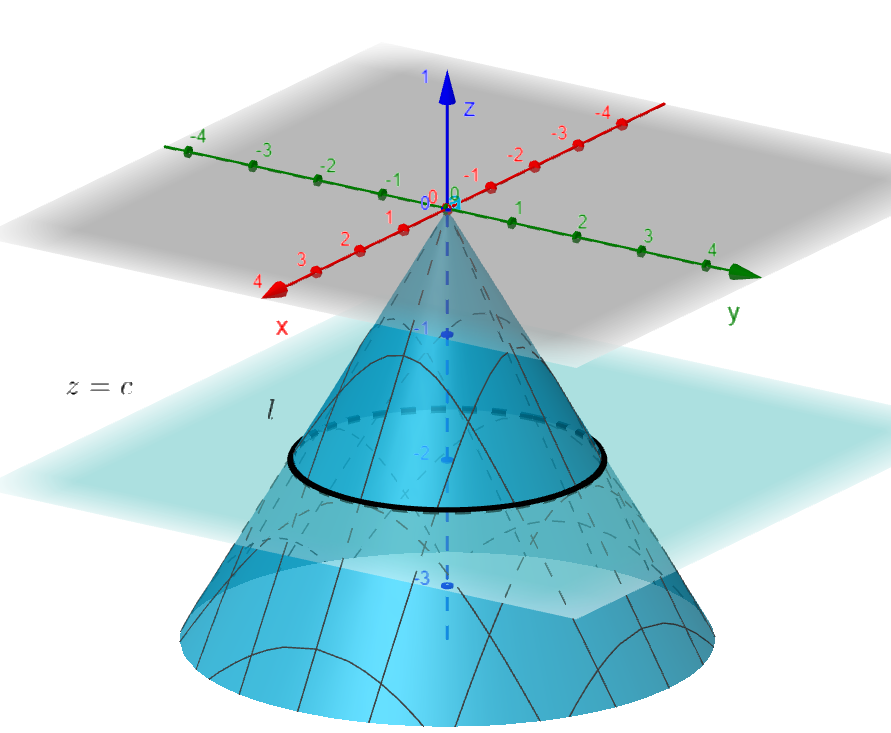
\includegraphics[height=90mm]{calculus/images/calculus_2024_03_13_1}

    Линии уровня $z = c$:

    \begin{enumerate}
        \item $c > 0 \quad \emptyset$
        \item $c = 0 \quad x = y = 0 - $ точка $(0, 0)$
        \item $c < 0 \quad -|c| = -\sqrt{x^2 + y^2} \quad c^2 = x^2 + y^2$
    \end{enumerate}


    \section{4.7.2. Производная по направлению, Градиент}

    Задача. Дано скалярное поле $u = u(x, y, z)$ (напр. давления). Как меняется давление при перемещении в заданном направлении?

    Это задача о нахождении скорости изменения $u(x, y, z)$ в заданном направлении $\overrightarrow{s}$

    Из $M_0(x_0, y_0, z_0)$ движемся в $M(x, y, z)$ в направлении $\overrightarrow{s}$, $x = x_0 + \Delta x$, $y = y_0 + \Delta y$, $z = z_0 + \Delta z$

    $\Delta s = \sqrt{(\Delta x)^2 + (\Delta y)^2 + (\Delta z)^2} \quad \Big| \cdot \frac{1}{\Delta s}$

    $1 = \sqrt{(\frac{\Delta x}{\Delta s})^2 + (\frac{\Delta y}{\Delta s})^2 + (\frac{\Delta z}{\Delta s})^2}$

    $(\frac{\Delta x}{\Delta s}, \frac{\Delta y}{\Delta s}, \frac{\Delta z}{\Delta s}) = (\cos\alpha, \cos\beta, \cos\gamma) = \overrightarrow{s^0}$

    Потребуем, чтобы $u(x, y, z)$ имела непрерывность $u_x, u_y, u_z$ в $D$

    То есть $u(x, y, z)$ дифференцируема и

    $\Delta u = du + o(\Delta s) = u_x \Delta x + u_y \Delta y + u_z \Delta x + o(\Delta s) \quad \Big| \cdot \frac{1}{\Delta s}$

    $\frac{\Delta u}{\Delta s} = u_x \cos\alpha + u_y \cos\beta + u_z \cos\gamma + \frac{o(\Delta s)}{\Delta s}$ - предельный переход

    $\frac{\partial u}{\partial s} = \frac{\partial u}{\partial x} \cos\alpha + \frac{\partial u}{\partial y} \cos\beta + \frac{\partial u}{\partial z} \cos\gamma$

    \Nota Изначально $\Delta u = du + \text{(б. м.)} \Delta x + \text{(б. м.)} \Delta y + \text{(б. м.)} \Delta z \quad \Big| \cdot \frac{1}{\Delta s}$

    $\frac{\Delta u}{\Delta s} = \frac{du}{\Delta s} + \text{(б. м.)} \cos\alpha$, $\text{(б. м.)} \cos\alpha \rightarrow 0$

    \Def $\frac{\partial u}{\partial s} = \frac{\partial u}{\partial x} \cos\alpha + \frac{\partial u}{\partial y} \cos\beta + \frac{\partial u}{\partial z} \cos\gamma$

    где $\alpha, \beta, \gamma$ - направления $\overrightarrow{s}$, называют производной функции $u = u(x, y, z)$ в направлении $\overrightarrow{s}$

    \Nota Производная в определении - число, но $\frac{\partial u}{\partial s} \overrightarrow{s^0}$ - вектор скорости

    \Nota Заметим, что если $\overrightarrow{i}, \overrightarrow{j}, \overrightarrow{k}$ - декартовы орты, то

    $\frac{\partial u}{\partial i} = \frac{\partial u}{\partial x} 1 + \frac{\partial u}{\partial y} 0 + \frac{\partial u}{\partial z} 0 = \frac{\partial u}{\partial x}$

    и аналогично в других направлениях: $\frac{\partial u}{\partial j} = \frac{\partial u}{\partial y}, \frac{\partial u}{\partial k} = \frac{\partial u}{\partial z}$

    Составим вектор $\frac{\partial u}{\partial x} \overrightarrow{i} + \frac{\partial u}{\partial y} \overrightarrow{j} + \frac{\partial u}{\partial z} \overrightarrow{k} \stackrel{\text{обозн}}{=} \overrightarrow{\triangledown} u$

    $\overrightarrow{\triangledown}$ - набла-оператор (оператор Гамильтона); $\overrightarrow{\triangledown} = (\frac{\partial}{\partial x}; \frac{\partial}{\partial y}; \frac{\partial}{\partial z})$ - условный вектор

    \Def $\overrightarrow{grad} \ u \stackrel{def}{=} \overrightarrow{\triangledown} u$ - называют градиентом функции $u(x, y, z)$

    Свойства градиентов:

    \ThN{1} $\frac{\partial u}{\partial s} = \text{пр.}_{\overrightarrow{s}} \overrightarrow{\triangledown} u$

    \ThN{2} $\overrightarrow{\triangledown} u$ - направление наибольшего значения $\frac{\partial u}{\partial s}$

    \ThN{3} $\overrightarrow{s} \perp \overrightarrow{\triangledown} u \Longrightarrow \frac{\partial u}{\partial s} = 0$

    \ThN{4} $u = u(x, y), u = c$ - линии уровня $l$. Тогда $\overrightarrow{\triangledown} u \perp l$

    Доказательства:

    \begin{enumerate}
        \item $\frac{\partial u}{\partial s} = (\frac{\partial}{\partial x}; \frac{\partial}{\partial y}; \frac{\partial}{\partial z}) \cdot \overrightarrow{s^0} =
        \overrightarrow{\triangledown} u \overrightarrow{s^0} = |\overrightarrow{\triangledown} u| |\overrightarrow{s^0}| \cos(\overrightarrow{\triangledown} u, \overrightarrow{s^0}) =
        |\overrightarrow{\triangledown} u| \cos(\overrightarrow{\triangledown} u, \overrightarrow{s^0}) = \text{пр.}_{\overrightarrow{s}} \overrightarrow{\triangledown} u$

        \item $\frac{\partial u}{\partial s} = |\overrightarrow{\triangledown} u| \cos\varphi \dots $ \Lab

        \item \Lab

        \item $u = c$ - уравнение $l_{\text{пр}}$ в плоскости $Oxy$, то есть $u(x, y) = c$, можем рассмотреть как неявную функцию $u(x, y(x)) - c = 0$

        Производная неявной функции: $\frac{dy}{dx} = -\frac{u_x}{u_y} = k_l$ - угловой коэффициент касательной к $l$

        $\overrightarrow{\triangledown} u = (u_x, u_y) \quad \frac{u_y}{u_x} = k_{\text{град.}}$ - наклон вектора градиента.
        Очевидно $k_l \cdot k_{\text{град.}} = -1 \Longrightarrow \overrightarrow{\triangledown} u \perp l$
    \end{enumerate}



    \Nota Итак, в теоремах сказано

    \textbf{1*} В любом заданном направлении $\overrightarrow{s}$ производная $\frac{\partial u}{\partial s} |_M$ равна проекции градиента в $M$

    \textbf{2-3*} В направлении $\overrightarrow{\triangledown} u$ производная $\frac{\partial u}{\partial s}$ наибольшая по модулю,
    а в направлении $\overrightarrow{s} \perp \overrightarrow{\triangledown} u$ $\frac{\partial u}{\partial s} = 0$

    \textbf{4*} Градиент $\perp$ линиям уровня.
    Прямая, содержащая $\overrightarrow{\triangledown} u$ (т. е. перпендикулярная касательной к $l$), называется нормалью к $l$
    а тогда $\overrightarrow{\triangledown} u$ - вектор нормали


    \section{4.7.3. Касательная и нормаль к поверхности}

    Будем исследовать поверхность $\pi$ с уравнением $F(x, y, z(x, y)) = 0$ (неявное задание)

    \Def Прямая $\tau$ называется касательной прямой к поверхности $\pi$ в точке $P(x, y, z)$,
    если эта прямая касается какой-либо кривой, лежащей на $\pi$ и проходящей через $P$

    \Nota Кривая получается (обычно) сечением $\pi$ какой-либо плоскостью

    \Nota В одной точке может быть множество касательных, но необязательно

    \Nota Договоримся различать два типа точек поверхности: обыкновенные и особые

    \Def Поверхность $\pi$ задана $F(x, y, z(x, y)) = 0$. Точка $M$ называется обыкновенной, если существуют
    все $\frac{\partial F}{\partial x}$, $\frac{\partial F}{\partial y}$, $\frac{\partial F}{\partial z}$,
    они непрерывны и не все равны нулю

    \Def Точка $M$ называется особой, если $\frac{\partial F}{\partial x} = \frac{\partial F}{\partial y} = \frac{\partial F}{\partial z} = 0$
    или хотя бы одна не существует

    \Th Все касательные прямые к $\pi$ в обыкновенной точке $M_0$ лежат в одной плоскости

    $\Box$

    $d \overrightarrow{s}$ - направляющий вектор касательной $\tau$, проведенной к кривой $l$ в некоторой секущей плоскости

    $d \overrightarrow{s}$ - вектор малых приращений, то есть $d \overrightarrow{s} = (dx, dy, dz)$

    $d \overrightarrow{p}$ - проекция $d \overrightarrow{s}$ на $Oxy$, то есть $d \overrightarrow{p} = (dx, dy)$

    Кривую $l$ можно задать параметрическими уравнениями $\begin{cases}x = \varphi(t) \\ y = \xi(t) \\ z = \theta(t)\end{cases}$

    Прямая $\tau$ имеет уравнение

    \[\frac{x - x_0}{dx} = \frac{y - y_0}{dy} = \frac{z - z_0}{dz}\]

    При отходе от $M_0$ на малое расстояние по поверхности (точнее по кривой $l$) задаем приращение $dt \neq 0$

    Домножим уравнение на $dt$

    \[\frac{x - x_0}{\frac{dx}{dt}} = \frac{y - y_0}{\frac{dy}{dt}} = \frac{z - z_0}{\frac{dz}{dt}}\]

    Из условия обыкновенности точки $M_0$ следует дифференцируемость функции $F$.
    Кроме того, уравнение можно преобразовать к виду $F(x(t), y(t), z(t)) = 0$, где $x(t), y(t), z(t)$ - тоже дифференцируемы в точке $M_0$

    Запишем $F^\prime_t$, как вложенную:

    \[F^\prime_t = \frac{\partial F}{\partial x}\frac{dx}{dt} + \frac{\partial F}{\partial y}\frac{dy}{dt} + \frac{\partial F}{\partial z}\frac{dz}{dt} = 0\]

    Или $\left(\frac{\partial F}{\partial x}, \frac{\partial F}{\partial y}, \frac{\partial F}{\partial z}\right) \cdot \left(\frac{dx}{dt}, \frac{dy}{dt}, \frac{dz}{dt}\right) = 0$

    Таким образом, $\overrightarrow{N} \cdot \frac{d\overrightarrow{s}}{dt} = 0$. То есть $\overrightarrow{N} \perp \frac{d\overrightarrow{s}}{dt}$, при том, что $d\overrightarrow{s}$ выбран произвольно (кривая $l$ - кривая произвольного сечения)

    Итак, вектор $\overrightarrow{N} \perp$ любой касательной $\tau$ к поверхности $\pi$ в точке $M_0$.
    Следовательно, все касательные лежат в плоскости $\kappa$ такой, что $\overrightarrow{N} \perp \kappa$

    $\Box$

    \Def Плоскость $\kappa$ (содержащая все касательные прямые $\tau$ к $\pi$ в точке $M_0$) называется касательной плоскостью к $\pi$ в $M_0$

    \Def Прямая в направлении $\overrightarrow{N}$ через точку $M_0$ называется нормалью к $\pi$ в $M_0$

    $\overrightarrow{N}$ - вектор нормали к поверхности в точке

    Уравнение ($\pi$) $\quad F(x, y, z) = 0, \ \overrightarrow{N} = \left(\frac{\partial F}{\partial x}, \frac{\partial F}{\partial y}, \frac{\partial F}{\partial z}\right), \ M_0(x_0, y_0, z_0) \in \pi, \kappa, n$

    Касательная плоскость ($\kappa$) $\quad \frac{\partial F}{\partial x} (x - x_0) + \frac{\partial F}{\partial y} (y - y_0) + \frac{\partial F}{\partial z} (z - z_0) = 0$

    Нормаль ($n$) $\quad \frac{x - x_0}{\frac{\partial F}{\partial x}} = \frac{y - y_0}{\frac{\partial F}{\partial y}} = \frac{z - z_0}{\frac{\partial F}{\partial z}}$

    \Nota Получим вектор нормали в случае явного задания $\pi \quad z = z(x, y)$

    Пересечем $\pi$ в точке $M_0$ плоскостями $x = x_0, y = y_0$.

    В сечении получим кривые с касательными векторами

    Вектор нормали к $\pi$ в $M_0 \quad \overrightarrow{n} = \overrightarrow{m} \times \overrightarrow{p}$

    Найдем $\overrightarrow{m}, \overrightarrow{p}$

    В сечении $x = x_0$

    картинка

    Введем вектор $d\overrightarrow{p} || \overrightarrow{p}$

    $d\overrightarrow{p} = \left(0, dy, \frac{\partial z}{\partial y}dy\right) = \left(0, 1, \frac{\partial z}{\partial y}\right) dy$

    Аналогично найдем $\overrightarrow{m}$ в сечении $y = y_0$

    $\overrightarrow{m} || d\overrightarrow{m} = \left(dx, 0, \frac{\partial z}{\partial x}dx\right) = \left(1, 0, \frac{\partial z}{\partial x}\right) dx$

    Так как модуль $\overrightarrow{n}$ не важен, а только направление, то будем искать
    $\overrightarrow{n} = \left(1, 0, \frac{\partial z}{\partial x}\right) \times \left(0, 1, \frac{\partial z}{\partial y}\right)$

    \[\overrightarrow{n} =
    \begin{vmatrix} \overrightarrow{i} & \overrightarrow{j} & \overrightarrow{k} \\
        1 & 0 & \frac{\partial z}{\partial x} \\ 0 & 1 & \frac{\partial z}{\partial y}
    \end{vmatrix} = \overrightarrow{i} \left(-\frac{\partial z}{\partial x}\right) - \overrightarrow{j} \frac{\partial z}{\partial y} + \overrightarrow{k} = \]

    \[= \left(-\frac{\partial z}{\partial x}; -\frac{\partial z}{\partial y}; 1\right)\]

    Тогда уравнение $\kappa$:

    \[z - z_0 = \frac{\partial z}{\partial x}(x - x_0) + \frac{\partial z}{\partial y} (y - y_0) = dz\]

    Уравнение нормали $n$: $\frac{x - x_0}{-\frac{\partial z}{\partial x}} = \frac{y - y_0}{-\frac{\partial z}{\partial y}} = \frac{z - z_0}{1}$

    \Nota Последние уравнения можно получить проще, если свести уравнение $z = f(x, y)$ к уравнению $z - f(x, y) = F(x, y, z) = 0$

    \Lab Вывести уравнение $\kappa$ и $n$, пользуясь предыдущим замечанием

    \Nota Если найти $\overrightarrow{n^-} = \overrightarrow{p} \times \overrightarrow{m} = - (\overrightarrow{m} \times \overrightarrow{p})$, то получим также вектор нормали, но обращенный в противоположную сторону

    Будем говорить, что $\overrightarrow{n^+}$ - положительный вектор нормали, если угол $\angle\gamma = \angle (\overrightarrow{n^+}, Oz) \in [0; \frac{pi}{2})$

    $\overrightarrow{n^-}$ - отрицательный, если угол $\angle\gamma = \angle (\overrightarrow{n^-}, Oz) \in \left(\frac{\pi}{2}; \pi\right)$

    Соответственно этому верхней стороной $\pi$ называется та, к которой вектор нормали положительный

    Нижней стороне соответствует $\overrightarrow{n^-}$

    Если $\overrightarrow{n} \perp Oz$, то это боковая сторона

    \section{4.7.4. Экстремумы ФНП (Ф$_2$П)}

    \Def Точка $M_0(x_0, y_0)$ называется точкой максимума (минимума) функции $z = z(x, y)$, если $\forall M \in U_\delta (M_0) \quad z(M_0) \geq z(M)$ (для минимума $z(M_0) \leq z(M)$)

    \Nota То же, что $z(M) - z(M_0) = z - z_0 = \Delta z \leq 0$ (max), $\quad \Delta z \geq 0$ (min)

    \Mem Для ФОП формулировали Необходимое условие экстремума (Ферма), из этого условия получали точки, подозрительные на экстремум : критические - $f^\prime(x_0) = 0$ или $\nexists f^\prime(x_0)$ (для острого экстремума); стационарные - $\exists f^\prime(x_0) = 0$ (частный случай критич.)

    Далее при помощи достаточных условий (признаков) проверяем наличие экстремума в критических точках

    \Nota Все термины переносятся на ФНП

    Необходимое условие и достаточное условие аналогично

    \Th Необходимое условие экстремума (гладкого):

    $z = z(x, y) : \Real^2 \rightarrow \Real$; $\quad z_0$ - точка гладкого экстремума,
    то есть $\exists \frac{\partial z}{\partial x}, \frac{\partial z}{\partial y}$ в $M_0$ и $\forall M \in U_\delta(M_0) \ z_0 \leq z(M)$ или $z_0 \geq z(M)$

    Тогда $\begin{cases}\frac{\partial z}{\partial x} |_{M_0} = 0 \\ \frac{\partial z}{\partial y} |_{M_0} = 0\end{cases}$

    $\Box$ Аналогично лемме Ферма в сечениях $x = x_0$, $y = y_0$ $\Box$

    Для существования острого экстремума нужно рассмотреть не существования или бесконечность $\frac{\partial z}{\partial x}$ или $\frac{\partial z}{\partial y}$

    Если же функция трижды дифференцируема исследования на характер экстремума можно проводить с помощью вторых производных

    \Th Достаточное условие (гладкого) экстремума

    Пусть $z = z(x, y)$ непрерывна в окрестности $x_0$ (критическая точка $\frac{\partial z}{\partial x} |_{M_0} = 0, \frac{\partial z}{\partial y} |_{M_0} = 0$)
    вместе со своими первыми и вторыми производными (можно потребовать трижды дифференцируемость)

    Тогда, если $\frac{\partial^2 z}{\partial x^2} \stackrel{\text{обозн}}{=} A, \frac{\partial^2 z}{\partial x \partial y} \stackrel{\text{обозн}}{=} B, \frac{\partial^2 z}{\partial y^2} \stackrel{\text{обозн}}{=} C$, то

    \begin{enumerate}
        \item $AC - B^2 > 0, A > 0 \Longrightarrow M_0$ - точка минимума
        \item $AC - B^2 > 0, A < 0 \Longrightarrow M_0$ - точка максимума
        \item $AC - B^2 < 0$ в точке $M_0$ нет экстремума
        \item $AC - B^2 = 0\Longrightarrow$ нельзя утверждать наличие или отсутствие экстремума в точке (требуются дополнительные исследования)
    \end{enumerate}

    $\Box$

    Функция $z$ дважды дифференцируема, тогда ($z_0 = z(M_0)$)

    $\Delta z = z - z_0 = \frac{dz}{1!} |_{M_0} + \frac{d^2 z}{2!} |_{M_0} + o((\Delta \rho)^2) \quad \Delta \rho = \sqrt{(\Delta x)^2 + (\Delta y)^2} = \sqrt{(dx)^2 + (dy)^2}, \ dx = \Delta\rho \cos\alpha, dy = \Delta\rho \sin\alpha$

    $o((\Delta \rho)^2) = \lambda (\Delta \rho)^3$

    Заметим, что $dz |_{M_0} = 0$, так как $M_0$ - критическая

    $d^2 z = \left(\frac{\partial}{\partial x} + \frac{\partial}{\partial y}\right)^2 z = \left(\frac{\partial^2}{\partial x^2} + 2 \frac{\partial^2}{\partial x \partial y} + \frac{\partial^2}{\partial y^2}\right) z =
    \frac{\partial^2 z}{\partial x^2} (dx)^2 + 2 \frac{\partial^2 z}{\partial x \partial y} dxdy + \frac{\partial^2 z}{\partial y^2} (dy)^2 = A (dx)^2 + 2B dxdy + C(dy)^2 =
    A(\Delta \rho)^2 \cos^2\alpha + 2B (\Delta \rho)^2 \cos\alpha\sin\alpha + C(\Delta \rho)^2 \sin^2\alpha$

    Тогда $\Delta z = \frac{1}{2} (\Delta \rho)^2 (A\cos^2\alpha + 2B\cos\alpha\sin\alpha + C\sin^2\alpha + 2\lambda \Delta \rho)$

    Далее рассмотрим отдельно случаи $A \neq 0$ и $A = 0$

    $A \neq 0$: $A\cos^2\alpha + 2B\cos\alpha\sin\alpha + C\sin^2\alpha = \frac{A^2\cos^2\alpha + 2AB\cos\alpha\sin\alpha + B^2\sin^2\alpha + (AC - B^2)\sin^2\alpha}{A} =
    \frac{(A\cos\alpha + B\sin\alpha)^2 + (AC - B^2)\sin^2\alpha}{A}$

    1) $\sqsupset AC - B^2 > 0 (A > 0)$: Числитель неотрицательный и не равен нулю (иначе $\sin\alpha = 0$, то тогда $A\cos\alpha \neq 0$)

    Итак, числитель и знаменатель больше нуля. Обозначим всю дробь за $k^2 > 0$

    Вернемся к $\Delta z = \frac{1}{2}(\Delta \rho)^2 (k^2 + 2\lambda\Delta\rho)$

    Устремим $\Delta \rho \rightarrow 0$, начиная с какого-то $\delta \ \forall M \in U_\delta(M_0) \ k^2 + \lambda\Delta\rho > 0$

    То есть $\Delta z > 0$ в $U_\delta(M_0) \Longrightarrow M_0$ - точка минимума (локально в $U_\delta(M_0)$)

    2) $\sqsupset AC - B^2 > 0 (A < 0)$, тогда $\Delta z = \frac{1}{2}(\Delta \rho)^2 (-k^2 + 2\lambda\Delta\rho) < 0$ при достаточно малом $\Delta \rho$

    3) $\sqsupset AC - B^2 < 0 (A > 0)$, тогда фиксируем направления $\alpha = 0 \Longrightarrow \sin\alpha = 0$

    $\Delta z = \frac{1}{2}(\Delta \rho)^2 (A + 2\lambda\Delta\rho) > 0$

    $tg \alpha = -\frac{A}{B} \Longrightarrow \frac{(AC - B^2)\sin^2\alpha}{A} = -k^2, \Delta z = \frac{(\Delta \rho)^2}{2}(-k^2 + 2\lambda\Delta\rho) < 0$

    Вдоль разных путей $\alpha = 0$, $tg \alpha = -\frac{A}{B}$, разный знак $\Delta z \Longrightarrow$ нет экстремума

    \Nota Можно аналогично рассмотреть $A < 0$

    4) $A = 0$, вернемся к выражению $\Delta z = \frac{1}{2} (\Delta \rho)^2 (\sin\alpha(2B\cos\alpha + C\sin\alpha) + 2\lambda\Delta\rho)$

    Пусть $\alpha$ беск. мал, тогда $\sin\alpha \approx 0, C\sin\alpha \approx 0, 2B\cos\alpha \approx 2B$. Тогда знак $\sin\alpha \cdot 2B$ зависит от $\alpha$

    То есть $\Delta z$ колеблется вместе с $\alpha$ по знаку $\Longrightarrow$ нет экстремума

    Можно доказать при $A \neq 0$, например, выбрав $tg \alpha = -\frac{A}{B}$, что знак $\Delta z$ зависит от $\alpha$

    $\Box$



    \clearpage


    \section{5. Интеграл ФНП}


    \section{5.1. Общая схема интегрирования}

    \underline{Постановка задачи.}

    В некоторой области $\Omega$ (дуга кривой, участок поверхности, тело и т. д.)
    распределена или действует непрерывно некоторая функция скалярная $g$ или векторная $\overrightarrow{G}$,
    то есть определены $g(M)$ или $\overrightarrow{G}$ $\forall M \in \Omega$

    \Ex Область $\Omega$ - дуга кривой $l : y = y(x)$

    Скалярная функция $g(M)$ - плотность в точке $M$

    \Ex Область $\Omega$ - трубка в $\Real^3$

    Векторная величина $\overrightarrow{G}(M)$ - скорость жидкой частицы, движущейся по трубке

    Из всех векторов $\overrightarrow{v}$ (для всех $M \in \Omega$) складывается \enquote{поле жидких скоростей}

    \Ex Область $\Omega$ - кривая, по которой движется точка $M$ под действием силы $\overrightarrow{G}(M)$

    Задача интегрирования - найти суммарное содержание скалярной величины или действие векторной величины в области $\Omega$

    \underline{Схема} Величины $g(M)$ и $\overrightarrow{G}(M)$, меняясь от точки к точке заменяются на квазипостоянные на малых (элементарных) участках $d\omega$

    Так как $g(M)$ или $\overrightarrow{G}(M)$ должны быть непрерывны на $\Omega$, то на малом участке $d\omega$ их изменение незначительно и
    значение функции можно считать почти постоянным, приняв за это значение какое-либо среднее $g_{\text{ср.}}(M), \overrightarrow{G_{\text{ср.}}}(M)$

    Тогда элементарное содержание $g(M)$ в $d\omega$ будет отличаться от среднего содержания, то есть $g_{\text{ср.}}d\omega$ на б. м. большего порядка

    \Ex Проиллюстрируем на примере $\int_a^b f(x) dx$

    $S$ - площадь по наибольшей границе, $\sigma$ - площадь по наименьшей границе, $S_{\text{трап.}}$ - \enquote{истинная} площадь

    Т. к. $f(x)$ непр. $\forall x \in [a, b]$, то $\Delta f \stackrel{\Delta x \to 0}{\rightarrow} 0$

    Для простоты рассмотрим монотонно возрастающую $f(x)$

    Хотим доказать, что $S - S_{\text{трап.}}$ - б. м. большего порядка, чем $S_{\text{трап.}}$ или $S$

    \[0 \leq S - S_{\text{трап.}} \leq dx \Delta y\]

    Сравним $\frac{dx \Delta y}{S} = \frac{dx \Delta y}{dx f(x + \Delta x)} = \frac{\Delta y}{\text{огр.}} \stackrel{\Delta x \to 0}{\rightarrow} 0$

    таким образом $S - S_{\text{трап.}} = 0 (S_{\text{трап.}})$

    \underline{Смысл интеграла} в случае векторной функции $\overrightarrow{G}(M)$

    Будем интегрировать только скалярные выражения вида $\overrightarrow{G}(M) \cdot d\overrightarrow{\omega}$ - скал. произведение векторов,
    где $d\overrightarrow{\omega}$ - ориентированный элемент $d\omega$

    \Ex Сила $\overrightarrow{F}(M)$ перемещает точку $M$ вдоль плоской кривой $l$. При этом сила совершает работу по перемещению
    (работа $A$ - скалярная величина)

    Известна формула для $\overrightarrow{F} = const$ и перемещения $\overrightarrow{s}$ по прямой: $A = \overrightarrow{F} \cdot \overrightarrow{s}$

    Разобьем дугу на элементы $dl \approx ds$ и ориентируем их (зададим направление перемещению $ds$)

    $dl = ds + o(dl)$, $d\overrightarrow{s}$ - вектор элем. перемещения, как правило, $ds$ направлен согласовано с $Ox$

    Элемент работы $dA = \overrightarrow{F} \cdot d\overrightarrow{s} = (F_x, F_y) \cdot (dx, dy) \stackrel{\text{обозн.}}{=}
    (P, Q) \cdot (dx, dy) = Pdx + Qdy$ - скаляр. Вся работа равна $A = \int dA$

    \Nota Ориентированный участок поверхности $d\overrightarrow{\sigma}$ - это размер участка $d\sigma$, умноженный на вектор нормали к участку $\overrightarrow{n}$,
    то есть $d\overrightarrow{\sigma} = \overrightarrow{n}d\sigma$

    \underline{Итак.} Схема интегрирования:

    \textbf{1*} Дробление области $\Omega$ на элементы $d\omega$
    \textbf{2*} Выбор постоянного значения функции на $d\omega$, то есть $g_{\text{ср.}}$ или $\overrightarrow{G_\text{ср.}}$
    \textbf{3*} Составление подынтегрального выражения $g_{\text{ср.}}d\omega$ или $\overrightarrow{G_\text{ср.}}d\overrightarrow{\omega}$
    \textbf{4*} \enquote{Суммирование} элементарных величин $\int gd\omega$ или $\int \overrightarrow{G}d\overrightarrow{\omega}$


    \section{5.2. Классификация интегралов}

    \textbf{1* По размерности $\Omega$}

    \begin{tabular}{p{8cm}p{8cm}}
        $n = 1$: * прямая (опред. интеграл $\int_a^b$)    & * кривая (криволинейный интеграл $\int_A^B$)                       \\

        $n = 2$: * плоскость (двойной интеграл $\iint_D$) & * поверхность, не криволинейная (поверхностный интеграл $\iint_S$) \\

        $n = 3$: * пространство $\Real^3$  \\
        (тройной $\iiint_V$ или $\iiint_T$)

    \end{tabular}


    \textbf{2* По виду функции}

    \begin{tabular}{p{8cm}p{8cm}}
        скалярная $g(M)$                            & векторная $\overrightarrow{G}(M)$         \\

        $n = 1$: определенный, криволинейный I рода & криволин. II рода (интегралы в проекциях) \\

        $n = 2$: двойной, поверхн. I рода            & поверхн. II рода                          \\

        $n = 3$: тройной
    \end{tabular}



    \section{5.3. Двойной и тройной интегралы}

    \indent \Nota Дадим строгое определение

    \begin{tabular}{p{0.45\textwidth}p{0.45\textwidth}}
        \Defs $z = z(x, y) \quad z : D \subset \Real^2 \rightarrow \Real$
        &
        \Mems $\int_a^b f(x) dx \quad\quad f(x) : [a, b] \rightarrow \Real^+$ \\
        1) Дробление на $[x_{i-1}, x_i]$ длиной $\Delta x$
        &
        1) Дробление на элементы $P_i$ прямыми $x = const, y = const$, $S_{P_i} = \Delta x_i \Delta y_i$ (дали $dx$, $dy$) \\
        2) Выбор средней точки $M_i(\xi_i, \eta_i)$, по значению $z(M_i)$ строим элемент. параллелепипед объемом

        $\nu_i = z(M_i) \Delta x_i \Delta y_i \approx V_{\text{малого цилиндра}}$
        &
        2) Выбор $\xi_i \in [x_{i-1}, x_i]$, площадь элементарных прямоугольников $f(\xi_i)\Delta x_i \approx S_{\text{полоски}}$ \\
        3) Интеграл суммы

        $v_i = \sum_{i=1}^n \nu_i = \sum z(M_i) \Delta x_i \Delta y_i$
        &
        3) Интеграл суммы $\sigma_n = \sum_{i=1}^n f(\xi_i) \Delta x_i$ \\
        4) Если $\exists \lim v_n \in \Real$, не зависящий от типа дробления и т.д. при $n \rightarrow \infty$ и
        $\tau = \max (\Delta x_i, \Delta y_i) \to 0$,

        то $\lim_{\substack{n\to\infty \\ \tau \to 0}} v_n \stackrel{def}{=} \iint_D z(x, y) dx dy$ - двойной интеграл от $z(x, y)$ на области $D$
        &
        4) $\lim_{\substack{n\to\infty \\ \tau \to 0}} \sigma_n = \int^b_a f(x) dx$

    \end{tabular}

    \Nota Об области $D$

    В простейшем случае рассматривают выпуклую, односвязную $\Real^2$-область

    a) Выпуклость:

    $\exists M_1, M_2 \in D \ | \ \overline{M_1 M_2} \notin D$ - не выпуклая

    $\forall M_1, M_2 \in D \ | \ \overline{M_1 M_2} \in D$ - выпуклая

    б) Связность:

    $D = D^\prime \union D^{\prime\prime}$ - не связная: $\exists M_1, M_2 \in D \ | \ \overset{\LARGE\smile}{M_1 M_2} \notin D$

    $D$ - связная: $\forall M_1, M_2 \in D \ | \ \overset{\LARGE\smile}{M_1 M_2} \in D$

    Обычно область - открытая, дальше будем рассматривать в том числе области с границей.

    Добавим к определению $\iint_{\partial D \text{ - граница } D} z(x, y) dx dy$

    Геометрический смысл: В определении при $z(x, y) \geq 0$ интегральная сумма $v_n = \sum_{i=1}^n \nu_i$ была суммой объемов элементарных параллелепипедов и приближала объем подповерхности

    Тогда $\iint_D z(x, y) dx dy \stackrel{z \geq 0}{=} V_{\text{цилиндра с осн. } D}$, а при $z = 1$ $\iint_D dx dy = S_D$

    Вычисление: По геометрическому смыслу найти $\iint_D z(x, y) dx dy$ - значит найти объем подповерхности

    Можно найти $S(x) = \int^{y_2(x)}_{y_1(x)} z(x = c, y) dy$ - площадь поперечного сечения

    Найдем $V$ как объем тела с известными площадями сечений

    $V = \int^b_a S(x) dx = \int_a^b \left(\int^{y_2(x)}_{y_1(x)} z(x = c, y) dy\right) dx$

    \Nota Кратный

    Если найдена первообразная для $z(x = c, y)$ (обозн. $F(x, y(x))$), то по формуле N-L:

    $\int^{y_2(x)}_{y_1(x)} z(x = c, y) dy = F(x, y(x)) \Big|^{y_2(x)}_{y_1(x)} = F(x, y_2(x)) - F(x, y_1(x))$

    Тогда $\int^b_a \stackrel{\varphi(x)}{\overgroup{(F(x, y_2) - F(x, y_1))}} dx$ - обычный определенный интеграл

    Пределы интегрирования во внутреннем интеграле - функции, во внешнем - точки

    ? Можно ли вычислить V, рассекая тело сечениями $y = const$? Верно ли, что $\int_a^b \left(\int_{y_1(x)}^{y_2(x)} z(x, y) dy\right) dx = \int_\alpha^\beta \left(\int_{x_1(y)}^{x_2(y)} z(x, y) dx\right) dy$?

    Верно, $V$ не зависит от порядка сечения

    Таким образом, двойной интеграл $\iint_D z(x, y) dxdy = \int_a^b \int_{y_1}^{y_2} z(x, y) dydx = \int_\alpha^\beta \int_{x_1}^{x_2} z(x, y) dxdy$

    Но при другом порядке интегрирования область $D$ может оказаться неправильной

    \Def При проходе области $D$ в направлении $Oy \uparrow$ граница области (верхняя) меняет аналитическое задание. Такая область называется неправильной в направлении $Oy$

    Выгодно выбирать правильное направление, чтобы не делить интеграл по аддитивности

    \Ex $\iint_D xy dx dy$, $D : x^2 + y^2 \leq 1$

    $\iint_D xy dx dy = \int_{-1}^1 \left(\int_{y_1 = -\sqrt{1-x^2}}^{y_2 = \sqrt{1-x^2}} xy dy\right) dx = \int_{-1}^1 \left(\frac{x}{2} y^2 \Big|_{y_1 = -\sqrt{1-x^2}}^{y_2 = \sqrt{1-x^2}}\right) dx =
    \int_{-1}^1 (\frac{x}{2} ((1 - x^2) - (1 - x^2)) dx = 0$

    \Def Тройной интеграл

    Пусть дана функция $u(x, y, z) \ : \ T \subset \Real^3 \rightarrow \Real$

    1) Дробление на элементы объема $dv = dxdydz$

    2) Вычисление среднего содержания $u(x, y, z)$ в $dv$: $u(\xi_i, \eta_i, \zeta_i) dv$

    3) Интегральная сумма $\sigma_n = \Sum u(M_i) dv$

    4) $\lim_{\substack{n \to \infty \\ \tau = \max (dv) \to 0}} \stackrel{def}{=} \iiint_T u(x, y, z) dxdydz$

    Геометрический смысл. Только при $u = 1$ интеграл $\iiint_T dxdydz = V_T$ равен объему

    Физический смысл. Пусть $u(x, y, z)$ - плотность в каждой точке $T$

    Тогда $\iiint_T u(x, y, z) dxdydz = m_T$ - масса

    Вычисление. $\iiint_T u(x, y, z) dxdydz \stackrel{\text{кратный}}{=} \int^b_a \int_{y_1(x)}^{y_2(x)} \int_{z_1(x, y)}^{z_2(x, y)} u(x, y, z) dz dy dx$



    \section{5.4. Замена переменной в двойном и тройном интегралах}

    Проблема. $S = \iint_D dxdy$

    Если $S_{D^\prime} = \int_0^{2\pi} d\varphi \int_0^R d\rho = \iint_{D^\prime} d\rho d\varphi$ - то это не площадь круга, а площадь прямоугольника $S$ в распрямленных координатах

    Введем $\Delta s_i$ - площадь кольцевого сектора в полярных координатах, а $\Delta s^\prime_i$ - площадь прямоугольника, причем $\Delta s_i \neq \Delta s_i^\prime$

    \Nota Будем искать поправочный коэффициент так, чтобы $\Delta s_i \approx \text{коэфф.} \cdot \Delta s_i^\prime$

    Дроблению будем подвергать область $D^\prime$ в распрямленной системе координат

    Введем новые криволинейные координаты: $\begin{cases}
                                                x = \varphi(u, v) \\ y = \psi(u, v)
    \end{cases}$,
    где функции $\varphi(u, v), \psi(u, v)$ непрерывно дифференцируемы по обоим аргументам

    Исходно область $D$ в $Oxy$

    картинка

    Заменим криволинейный параллелограмм на обычный, стянув вершины хордами (погрешность в площади - малая более высокого порядка, чем площадь)

    $A(x_A, y_A) = (\varphi(u, v), \psi(u, v))$

    $B(x_B, y_B) = (\varphi(u, v+\Delta v), \psi(u, v+\Delta v))$

    $C(x_C, y_C) = (\varphi(u + \Delta u, v+\Delta v), \psi(u + \Delta u, v+\Delta v))$

    $D(x_D, y_D) = (\varphi(u + \Delta u, v), \psi(u + \Delta u, v))$

    $S_{ABCD} = |\overrightarrow{AB} \cross \overrightarrow{AD}| = \left|
    \begin{vmatrix}
        \overrightarrow{i} & \overrightarrow{j} & \overrightarrow{k} \\
        x_B - x_A          & y_B - y_A          & 0                  \\
        x_D - x_A          & y_D - y_A          & 0
    \end{vmatrix}\right| = \left| \overrightarrow{k}
    \begin{vmatrix}
        x_B - x_A & y_B - y_A \\
        x_D - x_A & y_D - y_A
    \end{vmatrix}\right|$

    $x_B - x_A = \varphi(u, v + \Delta v) - \varphi(u, v) = \Delta_v \varphi \approx \frac{\partial \varphi}{\partial v}\Delta v$

    $y_B - y_A = \psi(u, v + \Delta v) - \psi(u, v) = \Delta_v \psi \approx \frac{\partial \psi}{\partial v}\Delta v$

    $x_D - x_A = \varphi(u + \Delta u, v) - \varphi(u, v) = \Delta_u \varphi \approx \frac{\partial \varphi}{\partial u}\Delta u$

    $y_D - y_A = \psi(u + \Delta u, v) - \psi(u, v) = \Delta_u \psi \approx \frac{\partial \psi}{\partial u}\Delta u$

    $\left| \overrightarrow{k}
    \begin{vmatrix}
        x_B - x_A & y_B - y_A \\
        x_D - x_A & y_D - y_A
    \end{vmatrix}\right| = \left|
    \begin{vmatrix}
        \frac{\partial \varphi}{\partial v}\Delta v & \frac{\partial \psi}{\partial v}\Delta v \\
        \frac{\partial \varphi}{\partial u}\Delta u & \frac{\partial \psi}{\partial u}\Delta u
    \end{vmatrix}\right| = \left|
    \begin{vmatrix}
        \frac{\partial \varphi}{\partial u} & \frac{\partial \varphi}{\partial u} \\
        \frac{\partial \psi}{\partial v}    & \frac{\partial \psi}{\partial u}
    \end{vmatrix}\right| \stackrel{\Delta s^\prime}{\overgroup{\Delta v \Delta u}} \stackrel{|det| = |J|}{\Longrightarrow} \Delta s \approx |J|\Delta s^\prime$

    \Nota В пределе это точное равенство:

    $|J| = \lim_{\Delta x \to 0} \frac{\Delta s}{\Delta s^\prime}$

    (легко понять, если считать частные приращения по теореме Лагранжа $\Delta_u \varphi = \frac{\partial \varphi}{\partial u}(\xi, \eta) \Delta u \rightarrow \frac{\partial \varphi}{\partial u}(u, v) \Delta u$)

    \Def Определитель $J = \begin{vmatrix}
                               \frac{\partial x_1}{\partial \xi_1} & \dots  & \frac{\partial x_1}{\partial \xi_n} \\
                               \vdots                              & \ddots & \vdots                              \\
                               \frac{\partial x_n}{\partial \xi_1} & \dots  & \frac{\partial x_n}{\partial \xi_n} \\
    \end{vmatrix}$, где $\begin{cases}
                             x_1 = f_1(\xi_1, \dots, \xi_n) \\
                             \dots \\
                             x_n = f_n(\xi_1, \dots, \xi_n) \\
    \end{cases}$ \begin{tabular}{r} - преобразование координат \\ $Ox_i \to O\xi_i (f_k \in C^1_D)$ \end{tabular}

    называется определителем Якоби или якобиан

    \vspace{5mm}

    \textbf{Построение интеграла.}
    \begin{enumerate}
        \item Дробление $D^\prime$ в распрямленной $Ouv$
        \item Выбор средней точки, поиск значения $f(\xi_i, \eta_i)$

        Значение величины на элементе $f(\xi_i, \eta_i) |J| du dv$
        \item Интегральная сумма $\sigma_n = \Sigma f(\xi_i, \eta_i) |J| du dv$
        \item В пределе интеграл $\iint_D f(x, y) dx dy = \iint_{D^\prime} f(u, v) |J| du dv$
    \end{enumerate}

    \vspace{5mm}

    \textbf{Якобианы в ПСК, ЦСК, СфСК}

    \begin{enumerate}
        \item ПСК: $\quad \begin{cases}
                              x = \rho\cos\varphi \\ y = \rho\sin\varphi
        \end{cases} \quad
        \begin{matrix}
            \frac{\partial x}{\partial \rho} = \cos\varphi & \frac{\partial x}{\partial \varphi} = -\rho\sin\varphi \\
            \frac{\partial y}{\partial \rho} = \sin\varphi & \frac{\partial y}{\partial \varphi} = \rho\cos\varphi
        \end{matrix}$

        $J = \begin{vmatrix}\cos\varphi & -\rho\sin\varphi \\ \sin\varphi & \rho\cos\varphi\end{vmatrix} =
        \rho \begin{vmatrix}\cos\varphi & -\sin\varphi \\ \sin\varphi & \cos\varphi\end{vmatrix} = \rho$

        \item ЦСК: $\quad \begin{cases}
                              x = \rho\cos\varphi \\ y = \rho\sin\varphi \\ z = z
        \end{cases} \quad J = \begin{vmatrix}\cos\varphi & -\rho\sin\varphi & 0 \\ \sin\varphi & \rho\cos\varphi & 0 \\ 0 & 0 & 1\end{vmatrix} = \rho$

        \item СфСК - \Lab
    \end{enumerate}

    \Ex $T: \begin{matrix}x^2 + y^2 = z^2 \\ x^2 + y^2 = z\end{matrix}$

    Конус в ЦСК: $\rho = z, z > 0$
    Параболоид в ЦСК: $\rho = \sqrt{z}, z > 0$

    $V_T = \iiint_T dxdydz = \iiint_{T^\prime}\rho d\rho d\varphi dz = \int_0^{2\pi} d\varphi \int_0^1 d \rho \int_{z_1 = \rho^2}^{z_2=\rho} \rho dz =
    2\pi \int_0^1 \rho z \Big|_{z_1 = \rho^2}^{z_2=\rho} d\rho = 2\pi \int_0^1 (\rho^2 - \rho^3) d\rho =
    2\pi (\frac{\rho^3}{3} - \frac{\rho^4}{4}) \Big|_0^1 = 2\pi (\frac{1}{3} - \frac{1}{4}) = \frac{\pi}{6}$

    \Lab $T: \begin{matrix}x^2 + y^2 + z^2 = 1 \\ \sqrt{x^2 + y^2} = z\end{matrix}$ - мороженка, считать в СфСК


    \section{5.5. Криволинейные интегралы}

    I рода. Область интегрирования - кривая $l = \stackrel{\HUGE\smile}{AB}$ (дуга) (начнем с плоской дуги)

    На $l$ действует скалярная функция $f(x, y)$ (физ. смысл - плотность, то есть имеем неоднородный кривой стержень)

    Задача в нахождении \enquote{суммарной} величины $f(x, y)$, то есть интеграла: \enquote{складываем} элементы $f_{\text{ср}}(x, y) dl$


    Обозн. Получаем $\int_l f(x, y)dl = \int_{AB} f(x, y)dl$



    \Nota В строгом определении интегральная сумма строится так:

    $\overset{\smile}{M_{i-1}M_i}$ - элементарная дуга

    $\Delta l_i$ - длина элемента

    $\Delta s_i$ - длина стягивающей дуги

    $\Delta l_i \approx \Delta s_i$

    $M_{\text{ср.}}(\xi_i, \eta_i)$ - ср. точка элемента

    \[\sigma_n = \overset{n}{\underset{i = 1}{\Sigma}} f(\xi_i, \eta_i) \Delta s_i\]

    \vspace{10mm}

    II рода. Задача (вычисление работы силы вдоль пути)

    Вдоль пути $\overset{\smile}{AB}$ действует сила $\overrightarrow{F} = (P(x, y), Q(x, y))$

    Найдем элементарную работу $dA = \overrightarrow{F}_{\text{ср.}} d\overrightarrow{s}$, где $d\overrightarrow{s}$ - элементарное приращение

    $d\overrightarrow{s} = (dx, dy) = (\cos\alpha ds, \sin\alpha ds)$

    $\overrightarrow{F}_{\text{ср.}}$ - значение силы на эл. участке в какой-либо его точке

    Тогда. $dA = (P(x, y), Q(x, y)) \cdot (dx, dy) = P(x, y)dx + Q(x, y)dy$

    $A = \int_{AB} dA = \int_{AB} Pdx + Qdy$ - интеграл II рода (в проекциях)

    \Nota В проекциях, потому что $F_x = P, F_y = Q$, таким образом скалярное произведение записано в проекциях

    При этом часто рассматривают по отдельности

    $\int_{AB} f(x, y) dx$ и $\int_{AB} g(x, y) dy$

    \Nota Связь интегралов I и II рода

    $\int_L Pdx + Qdy = \int_L (P, Q)(dx, dy) = \int_L (P, Q) (\cos\alpha, \cos\beta) \underset{\approx dl}{\undergroup{ds}} =
    \int_L (P\cos\alpha + Q\cos\beta)dl$

    Обозначим $\overrightarrow{\tau} = (\cos\alpha, \cos\beta)$

    По теореме Лагранжа $\exists (\xi, \eta) \in$ элементарной дуге, касательная которой параллельна $ds$

    Тогда $d\overrightarrow{s} = \overrightarrow{\tau}ds \approx \overrightarrow{\tau}dl$, где $\overrightarrow{\tau}$ - единичный вектор, касательной в $(\xi, \eta)$

    Тогда $\int_L Pdx + Qdy \stackrel{\text{пред. в вект. форме}}{=\joinrel=} \int_L \overrightarrow{F}\overrightarrow{\tau} dl =
    \int_L \overrightarrow{F}\underset{\text{ориент. эл. дуги}}{\undergroup{\overrightarrow{dl}}}$

    Свойства:

    \Nota Свойства, не зависящие от прохода дуги, аналогичны свойствам определенного интеграла

    Направление обхода.

    \begin{multicols}{2}
        I рода

        $\int_{AB} f(x, y)dl = \int_{BA} f(x, y)dl$

        II рода

        $\int_{AB}Pdx + Qdy = -\int_{BA}Pdx + Qdy$
    \end{multicols}

    \Def Часто рассматривают замкнутую дугу, называемую контур. Тогда интегралы обозначаются

    $\oint_K f dl$ и $\oint_K Pdx + Qdy$.

    Если $K$ (контур) обходят против ч. с., то обозн. $\oint_{K^+}$

    Вычисление. (Сведение к $\int_a^b dx$ или $\int_\alpha^\beta dy$ или $\int_\tau^T dt$)

    1) Параметризация дуги $L$:

    \begin{cases}
        x = \varphi(t) \\
        y = \psi(t)
    \end{cases} $\varphi, \psi \in C^1_{[\tau, T]}$

    \begin{matrix}
        A(x_A, y_A) = (\varphi(\tau), \psi(\tau)) \\
        B(x_B, y_B) = (\varphi(T), \psi(T))
    \end{matrix}

    При этом задании $L \quad y = y(x), x \in [a, b]$ или $x = x(y), y \in [\alpha, \beta]$ - частные случаи параметризации

    2) \begin{multicols}{2}
        I рода

        $\int_{L} f(x, y) dl \stackrel{dl = \sqrt{\varphi_t^{\prime 2} + \psi_t^{\prime 2}}|dt|}{=\joinrel=\joinrel=\joinrel}$

        $\int_\tau^T f(t) \sqrt{\varphi_t^{\prime 2} + \psi_t^{\prime 2}}|dt|$

        II рода

        $\int_{L = \overset{\smile}{AB}}Pdx + Qdy \stackrel{dx = \varphi_t^\prime dt, dy = \psi_t^\prime}{=\joinrel=\joinrel=\joinrel}
        $

        $\int_\tau^T f(t) (P\varphi^\prime + Q\varphi_\prime)dt|$

    \end{multicols}

    \Ex Дуга $L$ - отрезок прямой от $A(1, 1)$ до $B(3, 5)$

    1) $\int_{AB} (x + y) dl = \begin{bmatrix}AB: \frac{x - 1}{2} = \frac{y - 1}{4} \\
    \text{или} y = 2x - 1, x \in [1, 3] \\
    f(x, y) = x + 2x - 1 = 3x - 1 \\
    dl = \sqrt{1 + y^{\prime 2}}dx = \sqrt{5}dx\end{bmatrix} =
    \int_1^3 (3x - 1) \sqrt{5}dx = \sqrt{5} (\frac{3x^2}{2} - x) \Big|_1^3 = \sqrt{5}(12 - 2) = 10\sqrt{5}$

    2) $\int_{AB} (x + y) dx + (x + y) dy = \begin{bmatrix}x \uparrow^3_1, y \uparrow^5_1 \\
    y = 2x - 1, x = \frac{y + 1}{2} \\
    dx = dx, dy = dy\end{bmatrix} = \int_1^3 (x + 2x - 1) dx + \int^5_1 (\frac{y + 1}{2} + y) dy = \\
    (\frac{3x^2}{2} - x) \Big|_1^3 + \frac{1}{2} (\frac{3y^2}{2} + y) \Big|_1^5 = 10 + 20 = 30$

    \Th Формула Грина

    $D \subset R^2$ - прав. $\uparrow Ox, \uparrow Oy$

    $\Gamma_D$ - гладкая замкнутая кривая

    В области $D$ действует $\overrightarrow{F} = (P(x, y), Q(x, y))$ - непрерывные дифференциалы

    Тогда $\iint_D (\frac{\partial Q}{\partial x} - \frac{\partial P}{\partial y}) dxdy = \oint_{K^+} Pdx + Qdy$

    $\Box \iint_D (\frac{\partial Q}{\partial x} - \frac{\partial P}{\partial y}) dxdy =
    \iint_D \frac{\partial Q}{\partial x} dxdy - \iint_D \frac{\partial P}{\partial y} dxdy =
    \int^\beta_\alpha dy \int_{x=x_1(y)}^{x=x_2(y)} \frac{\partial Q}{\partial x} dx -
    \int^b_a dx \int_{y=y_1(x)}^{y=y_2(x)} \frac{\partial P}{\partial y} dy =
    \int^\beta_\alpha (Q(x, y)\Big|^{x=x_2(y)}_{x=x_1(y)})dy - \int^b_a (P(x, y)\Big|^{y=y_2(x)}_{y=y_1(x)})dx = \\
    \int_\alpha^\beta (Q(x_2(y), y) - Q(x_1(y), y)) dy - \int_a^b (P(x, y_2(x)) - P(x, y_1(x))) dx =
    \int_{NST}Q dy - \int_{NMT} Q dy - \int_{MTS} P dx + \int_{MNS}Pdx =
    \underset{\oint_{K^+}Qdy}{\undergroup{\int_{NST} Qdy + \int_{TMN} Qdy}} +
    \underset{\oint_{K^+}Pdx}{\undergroup{\int_{STM} Qdy + \int_{MNS} Qdy}} =
    \oint_{K^+} Pdx + Qdy$

    $\Box$



    \underline{Следствие}. $S_D = \frac{1}{2} \oint_K xdy - ydx$

    $\frac{\partial P}{\partial y} = \frac{\partial}{\partial y}(- \frac{y}{2}) = -\frac{1}{2},
    \frac{\partial Q}{\partial x} = \frac{\partial}{\partial x}(\frac{x}{2}) = \frac{1}{2}$

    Формула Грина: $\iint_D (\frac{\partial P}{\partial y} - \frac{\partial Q}{\partial x})dxdy = \iint_D (\frac{1}{2} - (\-\frac{1}{2}))dxdy =
    \iint_D dxdy = S_D \stackrel{\text{Ф. Гр.}}{=} \oint_{K^+} (-\frac{y}{2})dx + \frac{x}{2} dy$

    $\int$НЗП -  Интеграл, не зависящий от пути интегрирования.

    \Def $P, Q : D \subset \Real^2 \to \Real$, непрерывно дифференцируемы по 2-м переменным

    $\overset{\smile}{AB} \subset D \quad \forall M, N \in D$

    Параметризация $\overset{\smile}{AB}:
    \begin{cases}x = \varphi(t) \\ y = \psi(t)\end{cases}$ - $\varphi, \psi$ - непр. дифф (кусочно)

    $I = \int_{AB}Pdx + Qdy$ называется интегралом НЗП, если $\forall M, N \in D \quad \int_{AMB}Pdx + Qdy = \int_{ANB}Pdx + Qdy$

    \Nota Обозначают $\int_A^B Pdx + Qdy$ или $\int_{(x_2,y_2)}^{(x_1,y_1)} Pdx + Qdy$

    \Th Об интеграле НЗП

    В условиях def

    \begin{enumerate}[label=\Roman*.]

    \item $\int_{AB} Pdx + Qdy$ - инт. НЗП

    \item $\oint_K Pdx + Qdy = 0 \quad \forall K \subset D$

    \item $\frac{\partial P}{\partial y} = \frac{\partial Q}{\partial x} \ \forall M(x, y) \in D$

    \item $\exists \Phi(x, y) \ | \ d\Phi = P(x, y)dx + Q(x, y)dy$ в обл. $D$

    Причем $\Phi(x, y) = \int_{(x_0,y_0)}^{(x_1,y_1)}Pdx+Qdy$, где $(x_0, y_0), (x_1,y_1) \in D$

    \end{enumerate}

    Тогда $I \Longleftrightarrow II \Longleftrightarrow III \Longleftrightarrow IV$

    $\Box I \Longleftrightarrow II$

    $\fbox{\Longrightarrow}$ По def $\int$НЗП $\Longleftrightarrow$ \int_{AMB} = \int_{ANB}

    Рассмотрим $\int_{AMB} - \int_{ANB} = \int_{AMB} + \int_{BNA} = \oint_K = 0 \forall K \subset D$

    $\fbox{\Longleftarrow}$ Достаточно разбить $\oint_{K^+} = \int_{AMB} + \int_{BNA} = 0$

    Поскольку $\int_{AMB} + \int_{BNA} = 0$, то $\int_{AMB} - \int_{ANB} = 0$

    II $\Longleftrightarrow$ III

    $\fbox{\Longrightarrow} \oint_K = 0 \stackrel{?}{\Longrightarrow} \frac{\partial P}{\partial y} = \frac{\partial Q}{\partial x} \ \forall M(x, y) \in D$

    От противного $\quad \exists M_0(x_0, y_0) \in D \ | \ \frac{\partial P}{\partial y} \Big|_{M_0} \neq \frac{\partial Q}{\partial x} \Big|_{M_0} \Longleftrightarrow (\frac{\partial P}{\partial y} - \frac{\partial Q}{\partial x}) \Big|_{M_0} \neq 0$

    Для определенности $\letsymbol (\frac{\partial P}{\partial y} - \frac{\partial Q}{\partial x}) \Big|_{M_0} > 0$

    Тогда $\exists \delta > 0 \ | \ (\frac{\partial P}{\partial y} - \frac{\partial Q}{\partial x}) \Big|_{M_0} > \delta > 0$

    Выберем малую окрестность в точке $M_0$ ($U(M_0)$) и обозначим ее контур $\Gamma$

    Так как $P$ и $Q$ непр. дифф., $(\frac{\partial P}{\partial y} - \frac{\partial Q}{\partial x}) \Big|_{M_0} > 0$ в $U(M_0)$

    Формула Грина: $\iint_{U(M_0)} (\frac{\partial P}{\partial y} - \frac{\partial Q}{\partial x}) dxdy > \iint_{U(M_0)} \delta dxdy = \delta S_{U(M_0)} > 0$

    С другой стороны $\iint_{U(M_0)} (\frac{\partial Q}{\partial x} - \frac{\partial P}{\partial y})dxdy = \oint_{\Gamma^+} Pdx + Qdy = 0$

    Таким образом, возникаем противоречие

    $\fbox{\Longleftarrow} \frac{\partial Q}{\partial x} = \frac{\partial P}{\partial y} \forall M \in D$

    Тогда $\forall D^\prime \subset D \ \ \iint_{D^\prime} (\frac{\partial Q}{\partial x} - \frac{\partial P}{\partial y}) dxdy = 0 = \oint_{\Gamma_{D^\prime}} Pdx + Qdy \forall \Gamma_{D^\prime} \subset D$

    III \Longleftrightarrow IV

    $\fbox{\Longrightarrow} \frac{\partial Q}{\partial x} = \frac{\partial P}{\partial y} \Longrightarrow \exists \Phi(x, y)$

    Так как доказано $I \Longleftrightarrow III$, то докажем $I \Longrightarrow IV$

    $\int_{AM} Pdx + Qdy = \int^{M(x,y)}_{A(x_0,y_0)} Pdx + Qdy$ - НЗП $\forall A, M \in D$

    Обозн. $\int^{M(x,y)}_{A(x_0,y_0)} Pdx + Qdy - \Phi(x,y)$

    Докажем, что $d\Phi = Pdx + Qdy$

    Так как $d\Phi(x,y) = \frac{\partial \Phi}{\partial x}dx - \frac{\partial \Phi}{\partial y}dy$, то нужно доказать $\frac{\partial \Phi}{\partial x} = P(x, y), \frac{\partial \Phi}{\partial y} = Q(x, y)$

    $\frac{\partial \Phi}{\partial x} = \lim_{\Delta x \to 0}\frac{\Delta_x \Phi}{\Delta x} = $ [задали приращение вдоль $MM_1$] $ =
    \lim_{\Delta x \to 0} \frac{\Phi(x + \Delta x, y) - \Phi(x,y)}{\Delta x} = \\
    \lim_{\Delta x \to 0} \frac{\int^{M_1}_A Pdx + Qdy - \int^M_A Pdx + Qdy}{\Delta x} =
    \lim_{\Delta x \to 0} \frac{\int^M_A + \int^{M_1}_M - \int^M_A}{\Delta x} = \lim_{\Delta x \to 0} \frac{\int^{M_1}_M}{\Delta x} \stackrel{\text{НЗП}}{=}
    \lim_{\Delta x \to 0} \frac{\int_{(x,y)}^{(x + \Delta x, y)} P dx}{\Delta x} = [\text{по th Лагранжа } \exists \xi \in [x; x + \Delta x]] = \lim_{\Delta x \to 0} \frac{P(\xi, y) \Delta x}{\Delta x} =
    \lim_{\Delta x \to 0} P(\xi, y) = P(x, y)$

    Аналогично $\frac{\partial \Phi}{\partial y} = Q(x, y)$

    $\fbox{\Longleftarrow} d\Phi = Pdx + Qdy \stackrel{?}{\Longrightarrow} \frac{\partial Q}{\partial x} = \frac{\partial P}{\partial y}$

    Известно $P = \frac{\partial \Phi}{\partial x}, Q = \frac{\partial \Phi}{\partial y}$

    Тогда $\frac{\partial Q}{\partial x} = \frac{\partial^2 \Phi}{\partial x \partial y} = \frac{\partial^2 \Phi}{\partial y \partial x} = \frac{\partial P}{\partial y}$

    $\Box$

    \Nota $\Phi$ - первообразная для $Pdx + Qdy$:

    \Th Ньютона-Лейбница

    Выполнены условия th об интеграле НЗП

    Тогда $\int_A^B Pdx + Qdy = \Phi(B) - \Phi(A)$

    $\Box \int_A^B Pdx + Qdy \stackrel{\exists \Phi | d\Phi = Pdx + Qdy}{=} \int_A^B d\Phi(x, y) \stackrel{\text{параметр.} AB}{=}
    \int_\alpha^\beta d\Phi(t) = \Phi(t) \Big|_\alpha^\beta = \Phi(\beta) - \Phi(\alpha) = \Phi(B) - \Phi(A)$

    $\Box$

    \underline{Применение}

    \Ex $\int_{AB} (4 - \frac{y^2}{x^2})dx + \frac{2y}{x}dy$

    Проверим НЗП: $\frac{\partial Q}{\partial x} = \frac{\partial P}{\partial y}$: $\frac{\partial P}{\partial y} = -\frac{2y}{x^2}$, $\frac{\partial Q}{\partial x} -\frac{2y}{x^2}$ \Longleftrightarrow НЗП

    Найдем первообразную $\Phi(x, y)$ на все случаи жизни:

    $\Phi(x, y) = \int_{M_0(x_0, y_0)}^{M(x, y)} Pdx + Qdy$

    Выберем путь (самый удобный)

    $\Phi(x, y) = \int_{M_0}^{N} + \int_{N}^{M}$

    $\int_{M_0}^{N} \stackrel{y = 0, x_0 = 1, dy = 0}{=} \int_{(1, 0)}^{(x, 0)} 4 dx = 4x \Big|_{(1,0)}^{(x,0)} = 4x - 4$

    $\int_{N}^{M} \stackrel{dx = 0}{=} \int_{(x, 0)}^{(x, y)} \frac{2y}{x} dy = \frac{y^2}{x} \Big|_{(x,0)}^{(x,y)} = \frac{y^2}{x}$

    $\Phi(x, y) = 4x - 4 + \frac{y^2}{x} + C = 4x + \frac{y^2}{x} + C$

    Проверим: $\frac{\partial \Phi}{\partial x} = 4 - \frac{y^2}{x^2} = P$, $\frac{\partial \Phi}{\partial y} = \frac{2y}{x} = Q$

    Теперь можем искать $\int_{AB} \forall A, B \in D$ по N-L

    $\letsymbol A(1, 1), B(2, 2)$

    $\int_{AB} Pdx + Qdy = \Phi \Big|_A^B = \frac{y^2}{x} + 4x \Big|_{(1,1)}^{(2,2)} = \frac{4}{2} + 8 - 1 - 4 = 5$

    \Nota Функция $\Phi$ ищется в тех случаях, когда $\int_A^B Pdx + Qdy = \int^B_A (P, Q) (dx, dy) = A$ - работа силы, которая не зависит от пути

    (\Exs работа силы тяжести не зависит от пути, а силы трения - зависит)

    \Ex $\letsymbol \overrightarrow{F} = (P, Q) = (0, -mg)$

    $\Phi(x, y) = \int_O^M 0dx - mgdy = -\int_0^y mgdy = -mgy$ - потенциал гравитационного поля (или силы тяжести)



    \section{5.6. Поверхностные интегралы}

    \paragraph{1* Поверхностные интегралы I рода} (по участку поверхности)

    \underline{Задача}. Масса поверхности

    $u = u(x, y, z)$ - плотность (физ. смысл)

    Элементарная масса: $dm = u_{\text{ср.}}(\xi, \eta, \zeta) d\sigma$, $d\sigma$ - элемент поверхности

    $M = \iint_S dm = \iint_S u(x, y, z)$ - пов. инт. I рода

    \Def 1) Дробление $S$ на элементы $\Delta \sigma_k$ коорд. плоскостями $x = x_i, y = y_j$

    2) Ср. точка $(\xi_k, \eta_k, \zeta_k)$

    3) Инт. сумма $\nu_n = \sum_{k = 1}^{n} u(\xi_k, \eta_k, \zeta_k) \Delta \sigma_k$

    4) $\iint_S u(x, y, z) \Delta \sigma = \lim_{\substack{n \to \infty \\ \tau = \max \Delta \sigma_k \to 0}} \nu_n$ - поверхностный интеграл первого рода

    Свойства: Смена обхода поверхности $S$ не меняет знака интеграла: $\iint_{S^+} u d\sigma = \iint_{S^-} u d\sigma$

    \mediumvspace

    \underline{Вычисление}

    \Mems Вычисление $\int_L f(x, y) dl$

    1) Параметризация $L \quad \begin{cases}x = \varphi(t) \\ y = \psi(t)\end{cases} \quad t \in [\alpha, \beta]$

    2) $dl = \sqrt{\varphi^{\prime 2}(t) + \psi^{\prime 2}(t)} |dt|$

    3) $f(x, y) = \tilde{f}(t)$

    $\iint_L f(x, y)dl = \int_\alpha^\beta \tilde{f}(t) \sqrt{\varphi^{\prime 2}(t) + \psi^{\prime 2}(t)} |dt|$

    \underline{Поверхностный}

    $\iint_S u(x, y, z) d\sigma$

    1) Параметризация $S$: самая частая - $z = z(x, y), (x, y) \in D$ - пределы интегрирования

    2) $d\sigma = \sqrt{1 + \left(\frac{\partial z}{\partial x}\right)^2 + \left(\frac{\partial z}{\partial y}\right)^2} |dxdy|$, но т. к.
    в двойном интеграле договорились, что $dxdy > 0$ (площадь), модуль можно не ставить (область $D$ проходится в направлении против часовой стрелки)

    3) $u(x, y, z) = \tilde{u}(x, y, z(x, y)) = \tilde{u}(x, y)$

    $\iint_S u(x, y, z) d\sigma = \iint_{D^+} \tilde{u}(x, y) \sqrt{1 + z_x^{\prime 2} + z_y^{\prime 2}} dxdy$

    \Ex $S: \ x^2 + y^2 = z^2, z = 0, z = 1$

    $u(x, y, z) = z$

    $\iint_S zd\sigma =
    \begin{bmatrix}
        S: z = \sqrt{x^2 + y^2} \\
        D: \text{круг}, x^2 + y^2 = 1 \\
        d\sigma = \sqrt{1 + \frac{x^2}{x^2 + y^2} + \frac{y^2}{x^2 + y^2}} dxdy = \sqrt{2} dxdy \\
    \end{bmatrix} =
    \iint_D \sqrt{x^2 + y^2} \sqrt{2} dxdy = \sqrt{2} \int^{2\pi}_{0} d\varphi \int_{0}^{\rho} \rho \underset{|j|}{\undergroup{\rho}} d\rho = \sqrt{2} 2\pi \frac{\rho^3}{3} \Big|_0^1 = \frac{2\sqrt{2}\pi}{3}$

    \paragraph{2* II рода.} \\

    \underline{Задача}. Поток

    Будем говорить о потоке вектора $\overrightarrow{F} = (P, Q, R)$ через площадку $S$ в направлении нормали $\overrightarrow{n^+}$ или $\overrightarrow{n^-}$

    Если задано поле жидких скоростей, то потоком называют количество жидкости, протекающей через $S$ за время $\Delta t$

    В простой ситуации поток $\Pi = FS (\overrightarrow{F} \perp S, \overrightarrow{F} = const)$

    В общем случаем $\overrightarrow{F}$ - переменная, $S$ - искривленная и $\angle \overrightarrow{F}, S \neq \frac{\pi}{2}$

    Переходим к вычислению элементарного потока $d\Pi$

    $d\sigma$ - малый элемент поверхности (почти плоский)

    В пределах $d\sigma$ $\overrightarrow{F}$ меняется мало, за среднее берем $\overrightarrow{F} = (P, Q, R)$, где $P = P(x, y, z), Q = Q(x, y, z), R(x, y, z)$

    Разберемся с наклоном: если площадка перпендикулярна, то $d\Pi = F d\sigma$,
    но в нашем случае высота цилиндра равна $\text{пр.}_{\overrightarrow{n}} \overrightarrow{F} = (\overrightarrow{n}, \overrightarrow{F}) = F \cos\varphi$, где $\overrightarrow{n}$ - единичный вектор нормали, $\varphi$ - угол между нормалью и потоком,
    $d\Pi = (\overrightarrow{F}, \overrightarrow{n}) d\sigma = F_n d\sigma$

    Пусть $\overrightarrow{n} = (\cos\alpha, \cos\beta, \cos\gamma)$, тогда $d\Pi = (\overrightarrow{F}, (\cos\alpha, \cos\beta, \cos\gamma)) d\sigma =
    (P\cos\alpha, Q\cos\beta, R\cos\gamma)d\sigma$

    Итак, $\Pi = \iint_{S^{\overrightarrow{n}}} d\Pi = \iint_{S^{\overrightarrow{n}}} F_n d\sigma = \iint_{S^{\overrightarrow{n}}} (\overrightarrow{F}, \overrightarrow{n})d\sigma = \iint_{S^{\overrightarrow{n}}} (P\cos\alpha + Q\cos\beta + R\cos\gamma)d\sigma$

    Но, еще нет координатной записи подынтегрального выражения

    Спроектируем $d\sigma$ на координатные плоскости

    Сначала разрежем поверхность $S$ на элементы плоскостями $x = const, y = const$ (уточним форму $d\sigma$). Т. к. $d\sigma$ мал, то можно считать его плоским параллелограммом

    Тогда $\cos\gamma d\sigma = \pm dxdy$ ($\gamma$ - угол между нормалью и осью $Oz$)

    Нашли последнее слагаемое $\iint_{S^{\overrightarrow{n}}} R\cos\gamma d\sigma$ в исходном интеграле (I рода, т. к. по участку $d\sigma$)

    Найдем $\iint_{S^{\overrightarrow{n}}} Q\cos\beta d\sigma$, разобьем поверхность на участки $d\sigma$ плоскостями $x = const, y = const$

    Аналогично $\cos\beta d\sigma = \pm dxdz$

    Тогда в $\iint_{S^{\overrightarrow{n}}} P\cos\alpha d\sigma \quad \cos\alpha d\sigma = \pm dydz$

    Окончательно, поток $\Pi = \iint_{S^{\overrightarrow{n}}} \pm Pdydz \pm Qdxdz \pm Rdxdy = \iint_{S^{\overrightarrow{n}}} (P\cos\alpha + Q\cos\beta + R\cos\gamma) d\sigma$ - связь интегралов I и II рода

    \Nota Формулу интеграла можно получить еще так: $(\overrightarrow{F}, \overrightarrow{n})d\sigma = \overrightarrow{F}\overrightarrow{n}d\sigma = \overrightarrow{F}d\overrightarrow{\sigma}$, где $d\overrightarrow{\sigma} = (\pm dydz, \pm dxdz, \pm dxdy)$

    \DefN{Математическое}

    Определим $I = \iint_{S^{\overrightarrow{n}}} f(x, y, z) dxdy$

    $I = \lim_{\substack{n \to \infty \\ \tau = \max \Delta s_k \to 0}} \sum_{k=1}^n f(\xi_k, \eta_k, \zeta_k) \Delta s_k$ - поверхностный интеграл второго рода
    ($\Delta s_k = \Delta x\Delta y$ - любого знака, согласованного с обходом)

    Свойства: Меняет знак при смене обхода с $\overrightarrow{n}^+$ на $\overrightarrow{n}^-$

    \underline{Вычисление}

    1) Параметризация $S$ \quad для $\iint Rdxdy \quad z = z(x, y)$, для $\iint Qdxdz \quad y = y(x, z)$,

    для $\iint Pdydz \quad x = x(y, z)$

    Пределы интегрирования $D_{xy} = \text{пр.}_{Oxy} S$ и т. д.

    2) $dxdy \to \pm dxdy$, если обход $D_{xy}$ в направлении против часовой стрелки

    3) $R(x, y, z) = \tilde{R}(x, y, z(x, y)), \dots$




    Разберем пример поверхностного интеграла:

    \Exs $S_1:\ x^2 + y^2 = 1, \quad S_2: z = 0, \quad S_3: z = 1$

    $S = \bigunion_{i = 1}^3 S_i$ - цилиндр

    $\overrightarrow{F} = (P, Q, R) = (x, y, z)$

    $\iint_{S_{\text{внешн.}}} x dy dz + y dx dz + z dx dy = \iint_{S_1} + \iint_{S_2} + \iint_{S_3}$

    Так как проекции $S_2$ на $Oxz$ и $Oyz$ - отрезки, то $dxdz = 0$, $dydz = 0$

    $\iint_{S_2} xdydz + ydxdz + zdxdy = \iint_{S_2} zdxdy = 0$

    $\iint_{S_3} zdxdy \stackrel{z |_{S_3} = 1}{=} \iint_{S_3} dxdy \stackrel{\text{с "+", так как }\overrightaarrow{n_3} \uparrow\uparrow Oz}{=} \iint_{D_{xy}} dxdy = \pi$

    $\iint_{S_1} xdydz + ydxdz = \iint_{D^+_{yz}: x = \sqrt{1 - y^2}} xdydz + \left(-\iint_{D^-_{yz}: x = -\sqrt{1 - y^2}} xdydz\right) + \iint_{D^+_{xz}} ydxdz + \left(-\iint_{D^-_{xz}} ydxdz\right) = \dots$


    \section{5.7. Связь поверхностных интегралов с другими}

    \Th \hypertarget{gaussostrogradskyy}{Гаусса-Остроградского}

    $S_1\ : \ z = z_1(x, y),\ S_3\ :\ z = z_3(x, y),\ S_2\ : \ f(x, y) = 0$ (проекция на $Oxy$ - кривая)

    $S = \bigunion_{i = 1}^3 S_i$ - замкнута! и ограничивает тело $T$

    $P = P(x, y, z), Q = Q(x, y, z), R = R(x, y, z)$ - непр. дифф., действуют в области $\Omega \supset T$

    Тогда $\oiint_{S_{\text{внешн.}}} Pdydz + Qdxdz + Rdxdy = \iiint_T \left(\frac{\partial P}{\partial x} + \frac{\partial Q}{\partial y} + \frac{\partial R}{\partial z}\right) dxdydz$

    \Mem Формула Грина

    $\oint_K Pdx + Qdy = \iint_{D_{xy}} \left(\frac{\partial Q}{\partial x} - \frac{\partial Q}{\partial y}\right) dxdy$

    $\Box$

    Вычислим почленно $\iiint_T \left(\frac{\partial P}{\partial x} + \frac{\partial Q}{\partial y} + \frac{\partial R}{\partial z}\right) dv$

    $\iiint_T \left(\frac{\partial R(x, y, z)}{\partial z} dz\right) dxdy = \iint_{D_{xy}} R(x, y, z) \Big|_{z = z_1 (x, y)}^{z = z_3(x, y)} dxdy = \iint_{D_{xy}} (R(x, y, z_3(x, y)) - R(x, y, z_1(x, y))) dxdy =
    \underset{\text{двойной}}{\iint_{D_{xy}} R(x, y, z_3) dxdy} - \iint_{D_{xy}} R(x, y, z_1(x, y)) dxdy = \underset{\text{поверхностный}}{\iint_{S_3} R(x, y, z) dxdy} + \iint_{S_1} R(x, y, z) dxdy +
    \underset{\text{равен } 0\text{, т.к. } dxdy\ |_{S_2} = 0}{\iint_{S_2} R(x, y, z) dxdy} = \iint_{S_{\text{внешн.}}} Rdxdy$

    \smallvspace

    Аналогично остальные члены:

    $\iiint_T \frac{\partial Q}{\partial y} dxdydz = \iint_{S_{\text{внешн.}}} Qdxdz, \iiint_T \frac{\partial P}{\partial y} dxdydz = \iint_{S_{\text{внешн.}}} Pdxdz$

    $\Box$

    \Nota Если $\iint_{S_{\text{внутр}}}$, то $\iint_S = - \iiint_T$

    \Nota С учетом связи поверхностных интегралов $\iiint_T \left(\frac{\partial P}{\partial x} + \frac{\partial Q}{\partial y} + \frac{\partial R}{\partial z}\right) dv =
    \iint_S (P\cos\alpha + Q\cos\beta + R\cos\gamma) dv$

    \Th \hypertarget{stoks}{Стокса}

    Пусть $S : z = z(x, y)$ - незамкнутая поверхность, $L$ - контур, на которую она опирается

    $\text{пр}_{Oxy} L = K_{xy}, \quad \text{пр}_{Oxy} S = D_{xy}$

    В области $\Omega \supset S$ действуют функции $P, Q, R$ - непр. дифф.

    Тогда $\oint_{L^+} Pdx + Qdy + Rdz = \iint_{S^+} \left(\left(\frac{\partial R}{\partial y} - \frac{\partial Q}{\partial z}\right)\cos\alpha +
    \left(\frac{\partial P}{\partial z} - \frac{\partial R}{\partial x}\right)\cos\beta + \left(\frac{\partial Q}{\partial x} - \frac{\partial P}{\partial y}\right)\cos\gamma\right) d\sigma$

    $\Box$

    Найдем слагаемое $\oint_L P(x, y, z) dx \stackrel{\text{на } L\ : \ z = z(x, y)}{=\joinrel=\joinrel=\joinrel=}
    \oint_{K^+_{xy}} \tilde{P}(x, y, z(x, y)) dx = \oint_{K_{xy}} \tilde{P}dx + \tilde{Q}dy =
    \iint_{D_{xy}} \left(\frac{\partial \tilde{Q}}{\partial x} - \frac{\partial \tilde{P}}{\partial y}\right) dxdy =
    -\iint_{D_{xy}} \frac{\partial \tilde{P}(x, y)}{\partial y} dxdy =
    -\iint_{S^+} \frac{\partial P(x, y, z)}{\partial y} dxdy =
    -\iint_{S^+} \left(\frac{\partial P}{\partial y} + \frac{\partial P}{\partial z} \frac{\partial z}{\partial y}\right) dxdy =
    -\iint_{S^+} \left(\frac{\partial P}{\partial y}\cos\gamma + \frac{\partial P}{\partial z} (-\cos\beta)\right) d\sigma$

    $\overrightarrow{n} = \left(\frac{-\frac{\partial z}{\partial x}}{\sqrt{1 + z_x^{\prime 2} + z_y^{\prime 2}}}\right)$

    $\cos\gamma = \frac{1}{\sqrt{1 + z_x^{\prime 2} + z_y^{\prime 2}}}$

    Аналогично $\oint_L Qdy = \iint_{S^+} \left(\frac{\partial Q}{\partial x}\cos\gamma - \frac{\partial Q}{\partial z}\cos\alpha\right) d\sigma,
    \oint_L Rdz = \iint_{S^+} \left(\frac{\partial R}{\partial y}\cos\alpha - \frac{\partial R}{\partial x}\cos\beta\right) d\sigma$

    Остается сложить интегралы

    $\Box$

    \ExN{1} $(P, Q, R) = (x, y, z)$

    В \Exs пункте 5.6. (вычисление поверхностного):

    $\iint_{S_{\text{внешн}} \text{ - замкнута!}} xdydz + ydxdz + zdxdy = \iiint_T \left(\frac{\partial x}{\partial x} + \frac{\partial y}{\partial y} + \frac{\partial z}{\partial z}\right) dv = 3V_{\text{цил.}}$

    \ExN{2} Те же $P, Q, R$

    $\oint_L Pdx + Qdy + Rdz = \iint_{S} \left(\overset{= 0}{\overgroup{\left(\frac{\partial z}{\partial y} - \frac{\partial y}{\partial z}\right)}} \cos\alpha + 0 + 0\right) d\sigma$

    \clearpage


    \section{6. Теория поля}


    \section{6.1. Определения}

    \DefN{1} $\Omega \supset \Real^n \quad$ Функция $u \ : \ \Omega \to \Real$ называется скалярным полем в $\Omega$

    \DefN{2} Функция $\overrightarrow{F} = (F_1(\overrightarrow{x}), \dots, F_n(\overrightarrow{x})) : \Omega \to \Real^n$ называется векторным полем

    \Nota Далее будем рассматривать функции в $\Real^3$, то есть $u = u(x, y, z)$ и $\overrightarrow{F} = (P(x, y, z), Q(x, y, z), R(x, y, z))$

    \Nota Функции $u$ и $\overrightarrow{F}$ могут зависеть от вренмени $t$. Тогда эти поля называются нестационарными. В противном случае стационарными


    \section{6.2. Геометрические характеристики полей}

    $u = u(x, y, z)$: $l$ - линии уровня $u = const$

    $\overrightarrow{F} = (P, Q, R)$: $w$ - векторная линия, в каждой точке $w$ вектор $\overrightarrow{F}$ - касательная к $w$

    \underline{Векторная трубка} - совокупность непересекающихся векторных линий

    \Nota Отыскание векторных линий

    Возьмем $\overrightarrow{\tau}$ - элементарный касательный вектор, $\overrightarrow{\tau} = (dx, dy, dz)$

    Определение векторной линии: $\overrightarrow{\tau} || \overrightarrow{F} \quad \frac{dx}{P} = \frac{dy}{Q} = \frac{dz}{R}$ - система ДУ

    \Ex $\overrightarrow{F} = y \overrightarrow{i} - x \overrightarrow{j}, M_0 (1, 0)$ - ищем векторную линию $w \ni M_0$

    Задача Коши:

    $\begin{cases}
         \frac{dx}{y} = -\frac{dy}{x} \\
         y(1) = 0
    \end{cases} \Longleftrightarrow \begin{cases}
                                        xdx = -ydy \\
                                        y(1) = 0
    \end{cases} \Longleftrightarrow \begin{cases}
                                        x^2 = -y^2 + C \\
                                        y(1) = 0 \Longrightarrow C = +1
    \end{cases} \Longleftrightarrow x^2 + y^2 = 1 $


    \section{6.3. Дифференциальные характеристики}

    \Mems $\overrightarrow{\triangledown}u = \overrightarrow{grad}u = \left(\frac{\partial u}{\partial x}; \frac{\partial u}{\partial y}; \frac{\partial u}{\partial z}\right)$ - градиент скалярного поля

    $\overrightarrow{\triangledown} = \left(\frac{\partial}{\partial x}; \frac{\partial}{\partial y}; \frac{\partial}{\partial z}\right)$ - набла-оператор

    \Nota Для $\overrightarrow{\triangledown}$ определены действия:

    $\overrightarrow{\triangledown} \cdot \overrightarrow{a} = \frac{\partial a_1}{\partial x} + \frac{\partial a_2}{\partial y} + \frac{\partial a_3}{\partial z}$

    $\overrightarrow{\triangledown} \times \overrightarrow{a} =
    \begin{vmatrix}
        \overrightarrow{i}          & \overrightarrow{j}          & \overrightarrow{j}          \\
        \frac{\partial}{\partial x} & \frac{\partial}{\partial y} & \frac{\partial}{\partial z} \\
        a_1                         & a_2                         & a_3
    \end{vmatrix}$

    Причем $\overrightarrow{\triangledown} \cdot \overrightarrow{\triangledown} = \frac{\partial^2}{\partial x^2} + \frac{\partial^2}{\partial y^2} + \frac{\partial^2}{\partial z^2} = \triangle$ - лапласиан

    $\overrightarrow{\triangledown} \times \overrightarrow{\triangledown} = 0$

    \Nota $\triangle u = \underset{\text{часть волнового уравнения матфизики}}{\frac{\partial^2 u}{\partial x^2} + \frac{\partial^2 u}{\partial y^2} + \frac{\partial^2 u}{\partial z^2}} = 0$ - уравнение, определяющее гармоническую функцию $u(x, y, z)$, уравнение Лапласа

    \DefN{1} \hypertarget{divergencyya}{Дивергенция} поля (\textit{divergence} - расхождение)

    $div \overrightarrow{F} \stackrel{def}{=} \overrightarrow{\triangledown} \cdot \overrightarrow{F}$

    \DefN{2} \hypertarget{rotor}{Вихрь (ротор)} поля

    $rot \overrightarrow{F} \stackrel{def}{=} \overrightarrow{\triangledown} \times \overrightarrow{F}$

    \DefN{3} Если $rot \overrightarrow{F} = 0$, то $\overrightarrow{F}$ называется \hypertarget{bezvihrevoepole}{безвихревым} полем

    \DefN{4} Если $div \overrightarrow{F} = 0$, то $\overrightarrow{F}$ называется \hypertarget{solenoidalnoepole}{соленоидальным}

    \Nota Безвихревое поле имеет незамкнутые векторные линии, а вихревое - замкнутые

    \ThN{1} Свойство безвихревого поля

    $rot \overrightarrow{F} = 0 \Longleftrightarrow \exists u(x, y, z) \ | \ \overrightarrow{\triangledown}u = \overrightarrow{F}$

    $\Box$ \fbox{\Longrightarrow}

    $rot \overrightarrow{F} =
    \begin{vmatrix}
        \overrightarrow{i}          & \overrightarrow{j}          & \overrightarrow{j}          \\
        \frac{\partial}{\partial x} & \frac{\partial}{\partial y} & \frac{\partial}{\partial z} \\
        P & Q & R
    \end{vmatrix} = \left(\frac{\partial R}{\partial y} - \frac{\partial Q}{\partial z}\right)\overrightarrow{i} + \left(\frac{\partial P}{\partial z} - \frac{\partial R}{\partial x}\right)\overrightarrow{j} + \left(\frac{\partial Q}{\partial x} - \frac{\partial P}{\partial y}\right)\overrightarrow{k} = 0$

    $\Longleftrightarrow
    \begin{cases}
        \frac{\partial R}{\partial y} = \frac{\partial Q}{\partial z} \\
        \frac{\partial P}{\partial z} = \frac{\partial R}{\partial x} \\
        \frac{\partial Q}{\partial x} = \frac{\partial P}{\partial y}
    \end{cases}$

    Рассмотрим $u = u(x, y, z) \ | \ \frac{\partial u}{\partial x} = P, \frac{\partial u}{\partial y} = Q, \frac{\partial u}{\partial z} = R$ - удовлетворяет системе равенств

    $\overrightarrow{F} = (P, Q, R) = \left(\frac{\partial u}{\partial x}, \frac{\partial u}{\partial y}, \frac{\partial u}{\partial z}\right) = \overrightarrow{\triangledown} u$

    \fbox{\Longleftarrow} $\overrightarrow{F} = \overrightarrow{\triangledown}u$ - дана

    $rot \overrightarrow{F} = \overrightarrow{\triangledown} \times \overrightarrow{F} = \overrightarrow{\triangledown} \times (\overrightarrow{\triangledown} u) = (\overrightarrow{\triangledown} \times \overrightarrow{\triangledown}) u = 0$

    $\Box$

    \Nota Доказали, что если векторное поле является градиентом какого-то скалярного, то его вихрь равен нулю: $rot \overrightarrow{grad} u = 0$

    \Def $\overrightarrow{F} = \overrightarrow{\triangledown} u \quad$ Поле $u(x, y, z)$ называется потенциалом поля $\overrightarrow{F}$

    Таким образом, доказано, что безвихревое поле потенциально

    \ThN{2} Свойство соленоидального поля

    $div (rot \overrightarrow{F}) = 0$

    $\Box$

    $div (rot \overrightarrow{F}) = div \overrightarrow{a} = \overrightarrow{\triangledown} \overrightarrow{a} = \overrightarrow{\triangledown} (\overrightarrow{\triangledown} \times \overrightarrow{F}) = (\overrightarrow{\triangledown} \times \overrightarrow{\triangledown}) \cdot \overrightarrow{F} = 0$

    $\Box$

    \section{6.4. Интегральные характеристики. Теоремы теории поля}

    \Mems 1) Поток поля $\overrightarrow{F}: \Pi = \iint_S \overrightarrow{F}d\overrightarrow{\sigma}$

    \Def 2) Циркуляция поля $\overrightarrow{F}: \Gamma = \oint_L Pdx + Qdy + Rdz$

    \Nota Запишем \Ths на векторном языке

    1* \hypertarget{gaussostrogradskyyvector}{\textbf{Гаусса-Остроградского}}

    $\iint_S Pdydz + Qdxdz + Rdxdy = \iiint_T \left(\frac{\partial P}{\partial x} + \frac{\partial Q}{\partial y} + \frac{\partial R}{\partial z}\right) dxdydz$

    $\iint_S (P, Q, R) (dydx, dxdz, dxdy) = \iint_S (P, Q, R) (\cos\alpha d\sigma, \cos\beta d\sigma, \cos\gamma d\sigma) =
    \iint_S \overrightarrow{F} \overrightarrow{n} d\sigma = \iint_S \overrightarrow{F} d\overrightarrow{\sigma}$

    $\iiint_T \left(\frac{\partial P}{\partial x} + \frac{\partial Q}{\partial y} + \frac{\partial R}{\partial z}\right) dxdydz = \iiint_T (\overrightarrow{\triangledown} \overrightarrow{F}) = \iiint_T div \overrightarrow{F}$

    \fbox{$\iint_S \overrightarrow{F} d\overrightarrow{\sigma} = \iiint_T div \overrightarrow{F}$}

    \mediumvspace

    2* \hypertarget{stoksvector}{\textbf{Стокса}}

    $Pdx + Qdy + Rdz = \overrightarrow{F}d\overrightarrow{l}$

    $\oint_L \overrightarrow{F}d\overrightarrow{l} = \iint_S rot \overrightarrow{F} \overrightarrow{n} d\sigma = \iint_S rot \overrightarrow{F} d\overrightarrow{\sigma}$

    \mediumvspace

    3* \hypertarget{potentialvector}{\textbf{\Ths о потенциале}}

    $\forall L \ \oint_L \overrightarrow{F}d\overrightarrow{l} = 0 \Longleftrightarrow rot \overrightarrow{F} = 0 \Longleftrightarrow \exists u(x, y, z) \ | \ \overrightarrow{\triangledown} = \overrightarrow{F}$

    (см. \Ths интеграла НЗП)

    \Ex $\overrightarrow{F} = x\overrightarrow{i} + xy \overrightarrow{j}, L: x = y, x = -y, x = 1$

    По формуле Грина (Стокса) $\oint_L \overrightarrow{F} d\overrightarrow{l} = \iint_{D} \left(\frac{\partial Q}{\partial x} - \frac{\partial P}{\partial y}\right) dxdy =
    \iint_D y dxdy \quad rot \overrightarrow{F} \neq 0$

    $\oint_L xdx + xydy = \int_{L_1} + \int_{L_2} + \int_{L_3} = \int_0^1 (x + x^2) dx + \int_{-1}^1 y dy - \int_0^1 (x + x^2) dx = \int_{-1}^1 y dy = 0$

    \section{6.5. Механический смысл}

    1* Дивергенция

    Гаусс-Остроградский: $\iiint_T div \overrightarrow{F} dv = \Pi$

    \Ths о среднем: $\exists M_1 \in T \ | \ \iiint_T div \overrightarrow{F} dv = div \overrightarrow{F} \Big|_{M_1} \cdot V_T = \Pi$

    $div \overrightarrow{F} \Big|_{M_1} = \frac{\Pi}{V_T}$, точка $M_0, S$ и $T$ выбраны произвольно

    $\letsymbol V_T \to 0$, тогда $div \overrightarrow{F} \Big|_{M_1 \to M_0} = \lim_{V_T \to 0} \frac{\Pi}{V_T}$ - поток через границу бесконечно малого объема с центром $M_0$, отнесенный к $V_T$ - мощность источника в $M_0$

    Таким образом, дивергенция поля - мощность источников

    \Nota Смысл утверждения $div (rot \overrightarrow F) = 0$ - поле вихря свободно от источников

    \Nota Утверждение $rot (\overrightarrow{grad} u) = 0$ - поле потенциалов свободно от вихрей

    \mediumvspace

    2* Ротор

    Стокс $\iint_S rot \overrightarrow{F} d\overrightarrow{\sigma} = \Gamma$

    \Ths о среднем: $\exists M_1 : \iint_S rot \overrightarrow{F} d\overrightarrow{\sigma} = rot \overrightarrow{F} \Big|_{M_1} \cdot S = \Gamma$

    $rot \overrightarrow{F} \Big|_{M_1} = \frac{\Gamma}{S}$, будем стягивать $S$ к точке $M_0$ \Longrightarrow $rot \overrightarrow{F} \Big|_{M_0} = \lim_{S \to 0} \frac{\Gamma}{S}$ - циркуляция по б.м. контуру с центром $M_0$



    \Mem Дифф. хар.: $div \overrightarrow{F} = \overrightarrow{\trianlgedown} \overrightarrow{F}, rot \overrightarrow{F} = \overrightarrow{\trianlgedown} \times \overrightarrow{F}$

    Инт. хар.: $\Pi = \iint_S \overrightarrow{F} d\overrightarrow{\sigma}, \Gamma = \oint_L \overrightarrow{F} d\overrightarrow{l}$

    Мех. смысл: 1) $div \overrightarrow{F} \Big|_{M_0} = \lim_{V \to 0} \frac{\Pi}{V}$ - мощность точечного источника

    Г.-О.: поток через замкнутую поверхность равен суммарной мощности испочников внутри

    2) $rot \overrightarrow{F} \Big|_{M_0} = \lim_{S \to 0} \frac{\Gamma}{S}$ - циркуляция по б. м. контуру. Мех. смысл - ?

    3) Поток $\Pi$ - кол-во жидкости через площадку за единицу времени

    4) $\Gamma$ - ?

    \Nota Выясним смысл ротора и циркуляции на примере конкретного поля

    \Ex $\overrightarrow{F} = -\omega y \overrightarrow{i} + \omega x \overrightarrow{j}$ - поле линейных скоростей, вращающегося твердого тела, где $\overrightarrow{\omega} = const$ - угловая скорость

    Выберем контур $L$, ограничивающий область $S$

    Найдем $\Gamma_L = \oint_L \overrightarrow{F}d\overrightarrow{l} = \oint_L (-\omega y) dx + \omega x dy \stackrel{\text{Стокс}}{=}
    \iint_S rot \overrightarrow{F} \overrightarrow{n} d\sigma = \iint_S (\frac{\partial Q}{\partial x} - \frac{\partial P}{\partial y})\cos \gamma d\sigma =
    \iint_S 2\omega \cos \gamma d\sigma$

    Так как ротор сонаправлен оси $Oz$, получаем $\cos \gamma = 1$

    $\iint_S 2\omega \cos \gamma d\sigma = 2\omega \iint_S d\sigma = 2\omega S$

    Раньше в интеграле видно, что $rot \overrightarrow{F} \overrightarrow{n} \Longrightarrow |rot \overrightarrow{F}| = 2\omega$

    То есть механический смысл ротора - удвоенная угловая скорость вращающегося тела (или диска)

    \Nota Чтобы уточнить смысл $\Gamma$, рассмотрим такое же поле жидких скоростей (водоворот)

    $\overrightarrow{v} = -\omega y \overrightarrow{i} + \omega x \overrightarrow{j}$ и погруженное в него колесо с лопатками (водяная мельница)

    В качестве контура $L$ ерем обод колева, а его располагаем под углом $\gamma$ к вектору $\overrightarrow{\omega}$

    Все равно $\Gamma_L = \iint_S 2\omega \cos \gamma d\sigma = 2\omega\cos \gamma S$

    Если $\gamma = 0$, то $\Gamma_L = 2\omega S$ - максимальная мощность вращения нашей мельницы

    Если, например, $\gamma = \frac{\pi}{2}$, то $\Gamma_L = 0$ - колесо перпендикулярно полю, поэтому оно не вращается

    \section{6.6. Приложения к физике}

    1* Уравнение неразрывности (в гидромеханике)

    \Nota Здесь потребуются формулы:

    $\frac{du(x(t), y(t), z(t))}{dt} = \frac{\partial u}{\partial t} + \frac{\partial u}{\partial x}\frac{dx}{dt} + \dots$

    $\overrightarrow{\triangledown} \cdot (f\overrightarrow{F}) = \overrightarrow{\triangledown} f \cdot \overrightarrow{F} + f \cdot (\overrightarrow{\triangledown} \overrightarrow{F})$, где $f$ - скалярное поле, $\overrightarrow{F}$ - векторное поле

    \underline{Задача} Дано $\overrightarrow{F} = \rho \overrightarrow{v}$ - поле скоростей жидкости с весом $\rho = \rho(x, y, z, t)$

    Через площадку $dS$ за время $dt$ протекает $d\Pi = \rho v_n dt dS$ или за ед. времени $d\Pi = \rho v_n dS$

    Приращение жидкости за единицу времени $|dm| = |\frac{\partial \rho}{\partial t} dV|$

    Поток жидкости равен ее убыли в объеме $V$, то есть $\Pi = \oiint_S \rho v_n dS = -\iiint_V \frac{\partial \rho}{\partial t} dV$

    Применяя Г.-О.: $\Pi = \iiint_V \div (\rho \overrightarrow{v}) dV = -\iiint_V \frac{\partial \rho}{\partial t} dV \Longleftrightarrow \iiint_V (div (\rho \overrightarrow{v}) + \frac{\partial \rho}{\partial t}) dV = 0 \quad \forall V$ (поэтому подынт. функ. = 0)

    $\Longleftrightarrow \overrightarrow{\triangledown} (\rho \overrightarrow{v}) + \frac{\partial \rho}{\partial t} = 0$

    Учтем: $\frac{d \rho}{dt} = \frac{\partial \rho}{\partial t} +  \frac{\partial \rho}{\partial x} \frac{dx}{dt} +  \frac{\partial \rho}{\partial y} \frac{dy}{dt} +  \frac{\partial \rho}{\partial z} \frac{dz}{dt} = \frac{\partial \rho}{\partial t} + \overrightarrow{\triangledown} \rho \overrightarrow{v}$

    % TODO

    $\overrightarrow{\triangledown} (\rho \overrightarrow{v}) = \overrightarrow{\triangledown} \rho \cdot \overrightarrow{v} + \rho \overrightarrow{\triangledown} \overrightarrow{v} \Longleftrightarrow \overrightarrow{\triangledown} \rho \overrightarrow{v} = \overrightarrow{\triangledown} (\rho \overrightarrow{v}) - \rho \overrightarrow{\triangledown} \overrightarrow{v}$

    $\frac{d\rho}{dt} + \rho div \overrightarrow{v} = 0$ - уравнение неразрывности (при несжимаемой жидкости $div \overrightarrow{v} = 0$)

    2* Уравнения Максвелла

    Экспериментально: 1) $\int_L \overrightarrow{H} d\overrightarrow{l} = \iint_S \overrightarrow{r}d\overrightarrow{\sigma}$ - закон Био-Савара

    2) $\int_L \overrightarrow{E} d\overrightarrow{l} = -\frac{\partial}{\partial t} \iint_S \overrightarrow{B}d\overrightarrow{\sigma}$ - закон Фарадея

    где $\overrightarrow{H}$ - магнитная сила, $\overrightarrow{r}$ - полный ток, $\overrightarrow{E}$ - электрическая сила, $\overrightarrow{B}$ - магнитная индукция

    Максвелл: $\overrightarrow{r}$ = ток проводимости + ток смещения = $\lambda \overrightarrow{E} + \varepsilon \frac{\partial \overrightarrow{E}}{\partial t}$

    $\lambda$ - коэффициент проводимости, $\varepsilon, \mu$ - проницаемость

    1) $\oint_L \overrightarrow{H} d\overrightarrow{l} = \iint_S (\lambda \overrightarrow{E} + \varepsilon \frac{\partial \overrightarrow{E}}{\partial t}) d\overrightarrow{\sigma}$

    Стокс: $\iint_S rot \overrightarrow{H} d\overrightarrow{\sigma} - \iint_S (\lambda \overrightarrow{E} + \varepsilon \frac{\partial \overrightarrow{E}}{\partial t}) d\overrightarrow{\sigma} = 0$

    В векторной форме: $rot \overrightarrow{H} = (\lambda \overrightarrow{E} + \varepsilon \frac{\partial \overrightarrow{E}}{\partial t})$ - источники магнитного поля - токи проводимости и смещения

    2) $\oint_L \overrightarrow{E}d\overrightarrow{l} = \iint_S rot \overrightarrow{E}d\overrightarrow{\sigma} = -\iint_S \frac{\partial \overrightarrow{B}}{\partial t}d\overrightarrow{\sigma} \Longleftrightarrow
    rot \overrightarrow{E} = -\frac{\partial \overrightarrow{B}}{\partial t}$ - изменение индукции дает эл. ток в соленоиде.

    3) $\overrightarrow{\triangledown} \varepsilon \overrightarrow{E} = \rho$

    4) $\overrightarrow{\triangledown} \mu \overrightarrow{H} = 0$




\end{document}

